\documentclass[a4paper]{report}
\usepackage[utf8]{inputenc}
\usepackage[T1]{fontenc}
\usepackage{RJournal}
\usepackage{amsmath,amssymb,array}
\usepackage{booktabs}
\usepackage{bm}

\let\hat\widehat
\let\tilde\widetilde
\let\check\widecheck
\def\given{{\,|\,}}
\def\ds{\displaystyle}
\newcommand\wtilde{\stackrel{\sim}{\smash{\mathcal{W}}\rule{0pt}{1.1ex}}}

%----- bold fonts -----%

\newcommand{\ab}{\mathbf{a}}
\newcommand{\bbb}{\mathbf{b}}
\newcommand{\cbb}{\mathbf{c}}
\newcommand{\db}{\mathbf{d}}
\newcommand{\eb}{\mathbf{e}}
\newcommand{\fb}{\mathbf{f}}
\newcommand{\gb}{\mathbf{g}}
\newcommand{\hb}{\mathbf{h}}
\newcommand{\ib}{\mathbf{i}}
\newcommand{\jb}{\mathbf{j}}
\newcommand{\kb}{\mathbf{k}}
\newcommand{\lb}{\mathbf{l}}
\newcommand{\mb}{\mathbf{m}}
\newcommand{\nbb}{\mathbf{n}}
\newcommand{\ob}{\mathbf{o}}
\newcommand{\pb}{\mathbf{p}}
\newcommand{\qb}{\mathbf{q}}
\newcommand{\rb}{\mathbf{r}}
\newcommand{\sbb}{\mathbf{s}}
\newcommand{\tb}{\mathbf{t}}
\newcommand{\ub}{\mathbf{u}}
\newcommand{\vb}{\mathbf{v}}
\newcommand{\wb}{\mathbf{w}}
\newcommand{\xb}{\mathbf{x}}
\newcommand{\yb}{\mathbf{y}}
\newcommand{\zb}{\mathbf{z}}

\newcommand{\ba}{\bm{a}}
\newcommand{\bb}{\bm{b}}
\newcommand{\bc}{\bm{c}}
\newcommand{\bd}{\bm{d}}
\newcommand{\be}{\bm{e}}
\newcommand{\bbf}{\bm{f}}
\newcommand{\bg}{\bm{g}}
\newcommand{\bh}{\bm{h}}
\newcommand{\bi}{\bmf{i}}
\newcommand{\bj}{\bm{j}}
\newcommand{\bk}{\bm{k}}
\newcommand{\bl}{\bm{l}}
\newcommand{\bbm}{\bm{m}}
\newcommand{\bn}{\bm{n}}
\newcommand{\bo}{\bm{o}}
\newcommand{\bp}{\bm{p}}
\newcommand{\bq}{\bm{q}}
\newcommand{\br}{\bm{r}}
\newcommand{\bs}{\bm{s}}
\newcommand{\bt}{\bm{t}}
\newcommand{\bu}{\bm{u}}
\newcommand{\bv}{\bm{v}}
\newcommand{\bw}{\bm{w}}
\newcommand{\bx}{\bm{x}}
\newcommand{\by}{\bm{y}}
\newcommand{\bz}{\bm{z}}




\newcommand{\Ab}{\mathbf{A}}
\newcommand{\Bb}{\mathbf{B}}
\newcommand{\Cb}{\mathbf{C}}
\newcommand{\Db}{\mathbf{D}}
\newcommand{\Eb}{\mathbf{E}}
\newcommand{\Fb}{\mathbf{F}}
\newcommand{\Gb}{\mathbf{G}}
\newcommand{\Hb}{\mathbf{H}}
\newcommand{\Ib}{\mathbf{I}}
\newcommand{\Jb}{\mathbf{J}}
\newcommand{\Kb}{\mathbf{K}}
\newcommand{\Lb}{\mathbf{L}}
\newcommand{\Mb}{\mathbf{M}}
\newcommand{\Nb}{\mathbf{N}}
\newcommand{\Ob}{\mathbf{O}}
\newcommand{\Pb}{\mathbf{P}}
\newcommand{\Qb}{\mathbf{Q}}
\newcommand{\Rb}{\mathbf{R}}
\newcommand{\Sbb}{\mathbf{S}}
\newcommand{\Tb}{\mathbf{T}}
\newcommand{\Ub}{\mathbf{U}}
\newcommand{\Vb}{\mathbf{V}}
\newcommand{\Wb}{\mathbf{W}}
\newcommand{\Xb}{\mathbf{X}}
\newcommand{\Yb}{\mathbf{Y}}
\newcommand{\Zb}{\mathbf{Z}}

\newcommand{\bA}{\bm{A}}
\newcommand{\bB}{\bm{B}}
\newcommand{\bC}{\bm{C}}
\newcommand{\bD}{\bm{D}}
\newcommand{\bE}{\bm{E}}
\newcommand{\bF}{\bm{F}}
\newcommand{\bG}{\bm{G}}
\newcommand{\bH}{\bm{H}}
\newcommand{\bI}{\bm{I}}
\newcommand{\bJ}{\bm{J}}
\newcommand{\bK}{\bm{K}}
\newcommand{\bL}{\bm{L}}
\newcommand{\bM}{\bm{M}}
\newcommand{\bN}{\bm{N}}
\newcommand{\bO}{\bm{O}}
\newcommand{\bP}{\bm{P}}
\newcommand{\bQ}{\bm{Q}}
\newcommand{\bR}{\bm{R}}
\newcommand{\bS}{\bm{S}}
\newcommand{\bT}{\bm{T}}
\newcommand{\bU}{\bm{U}}
\newcommand{\bV}{\bm{V}}
\newcommand{\bW}{\bm{W}}
\newcommand{\bX}{\bm{X}}
\newcommand{\bY}{\bm{Y}}
\newcommand{\bZ}{\bm{Z}}


%----- calligraphic fonts -----%

\newcommand{\cA}{\mathcal{A}}
\newcommand{\cB}{\mathcal{B}}
\newcommand{\cC}{\mathcal{C}}
\newcommand{\cD}{\mathcal{D}}
\newcommand{\cE}{\mathcal{E}}
\newcommand{\cF}{\mathcal{F}}
\newcommand{\cG}{\mathcal{G}}
\newcommand{\cH}{\mathcal{H}}
\newcommand{\cI}{\mathcal{I}}
\newcommand{\cJ}{\mathcal{J}}
\newcommand{\cK}{\mathcal{K}}
\newcommand{\cL}{\mathcal{L}}
\newcommand{\cM}{\mathcal{M}}
\newcommand{\cN}{\mathcal{N}}
\newcommand{\cO}{\mathcal{O}}
\newcommand{\cP}{\mathcal{P}}
\newcommand{\cQ}{\mathcal{Q}}
\newcommand{\cR}{\mathcal{R}}
\newcommand{\cS}{{\mathcal{S}}}
\newcommand{\cT}{{\mathcal{T}}}
\newcommand{\cU}{\mathcal{U}}
\newcommand{\cV}{\mathcal{V}}
\newcommand{\cW}{\mathcal{W}}
\newcommand{\cX}{\mathcal{X}}
\newcommand{\cY}{\mathcal{Y}}
\newcommand{\cZ}{\mathcal{Z}}




%----- blackboard bold fonts-----%

\newcommand{\CC}{\mathbb{C}}
\newcommand{\EE}{\mathbb{E}}
\newcommand{\GG}{\mathbb{G}}
\newcommand{\VV}{\mathbb{V}}
\newcommand{\II}{\mathbb{I}}
\newcommand{\KK}{\mathbb{K}}
\newcommand{\LL}{\mathbb{L}}
\newcommand{\MM}{\mathbb{M}}
\newcommand{\NN}{\mathbb{N}}
\newcommand{\PP}{\mathbb{P}}
\newcommand{\QQ}{\mathbb{Q}}
\newcommand{\RR}{\mathbb{R}}
\newcommand{\SSS}{\mathbb{S}}
\newcommand{\ZZ}{\mathbb{Z}}
\newcommand{\XX}{\mathbb{X}}
\newcommand{\YY}{\mathbb{Y}}
\newcommand{\OOmega}{\mathbb{\Omega}}



%%%%%bold greeks%%%%%
\newcommand{\bell} {\bm{\ell}}

%----- bold greek fonts -----%

\newcommand{\balpha}{\bm{\alpha}}
\newcommand{\bbeta}{\bm{\beta}}
\newcommand{\bgamma}{\bm{\gamma}}
\newcommand{\bepsilon}{\bm{\epsilon}}
\newcommand{\bvarepsilon}{\bm{\varepsilon}}
\newcommand{\bzeta}{\bm{\zeta}}
\newcommand{\btheta}{\bm{\theta}}
\newcommand{\bvartheta}{\bm{\vartheta}}
\newcommand{\bkappa}{\bm{\kappa}}
\newcommand{\blambda}{\bm{\lambda}}
\newcommand{\bmu}{\bm{\mu}}
\newcommand{\bnu}{\bm{\nu}}
\newcommand{\bxi}{\bm{\xi}}
\newcommand{\bpi}{\bm{\pi}}
\newcommand{\bvarpi}{\bm{\varpi}}
\newcommand{\brho}{\bm{\varrho}}
\newcommand{\bsigma}{\bm{\sigma}}
\newcommand{\bvarsigma}{\bm{\varsigma}}
\newcommand{\btau}{\bm{\tau}}
\newcommand{\bupsilon}{\bm{\upsilon}}
\newcommand{\bphi}{\bm{\phi}}
\newcommand{\bvarphi}{\bm{\varphi}}
\newcommand{\bchi}{\bm{\chi}}
\newcommand{\bpsi}{\bm{\psi}}
\newcommand{\bomega}{\bm{\omega}}

\newcommand{\bGamma}{\bm{\Gamma}}
\newcommand{\bDelta}{\bm{\Delta}}
\newcommand{\bTheta}{\bm{\Theta}}
\newcommand{\bLambda}{\bm{\Lambda}}
\newcommand{\bXi}{\bm{\Xi}}
\newcommand{\bPi}{\bm{\Pi}}
\newcommand{\bSigma}{\bm{\Sigma}}
\newcommand{\bUpsilon}{\bm{\Upsilon}}
\newcommand{\bPhi}{\bm{\Phi}}
\newcommand{\bPsi}{\bm{\Psi}}
\newcommand{\bOmega}{\bm{\Omega}}


%----- Some standard definitions -----%

\newcommand{\argmin}{\mathop{\mathrm{argmin}}}
\newcommand{\argmax}{\mathop{\mathrm{argmax}}}
\newcommand{\minimize}{\mathop{\mathrm{minimize}}}

\newcommand{\sign}{\mathop{\mathrm{sign}}}
\newcommand{\tr}{\mathop{\mathrm{tr}}}

\DeclareMathOperator{\Var}{{\rm Var}}
\DeclareMathOperator{\Cor}{\rm Corr}
\DeclareMathOperator{\Cov}{\rm Cov}
\DeclareMathOperator{\ind}{\mathds{1}}  % Indicator
\newcommand{\smallfrac}[2]{{\textstyle \frac{#1}{#2}}}  
                                                        
\newcommand*{\zero}{{\bm 0}}
\newcommand*{\one}{{\bm 1}}

\newcommand{\diag}{{\rm diag}}


%%%%%%%%%%%%%%%%%%%%%%%%%%%%%%%%%%%%%%


%%%%% Norms

%\newcommand{\norm}[1]{||#1||}
\newcommand{\bignorm}[1]{\bigg|\bigg|#1\bigg|\bigg|}
\newcommand{\opnorm}[2]{| \! | \! | #1 | \! | \! |_{{#2}}}

%%%%% Dot product
\newcommand{\dotp}[2]{\langle{#1},{#2}\rangle}

%%%%  brackets
\newcommand{\inner}[2]{\left\langle #1,#2 \right\rangle}
\newcommand{\rbr}[1]{\left(#1\right)}
\newcommand{\sbr}[1]{\left[#1\right]}
\newcommand{\cbr}[1]{\left\{#1\right\}}
\newcommand{\nbr}[1]{\left\|#1\right\|}
\newcommand{\abr}[1]{\left|#1\right|}

%%%%%%%%%  Other commands

\newcommand{\mcomment}[1]{\marginpar{\tiny{#1}}}
\newcommand{\fcomment}[1]{\footnote{\tiny{#1}}}
\newcommand{\overbar}[1]{\mkern 1.5mu\overline{\mkern-1.5mu#1\mkern-1.5mu}\mkern 1.5mu}
\newcommand{\ud}{{\,\mathrm{d}}}



\def\skeptic{{\sc skeptic}}
\newcommand{\sgn}{\mathop{\mathrm{sign}}}
\providecommand{\norm}[1]{\|#1\|}
\providecommand{\bnorm}[1]{\big\|#1\big\|}
\providecommand{\enorm}[1]{| \! | \! |#1| \! | \! |}
\providecommand{\bemnorm}[1]{\big| \! \big| \! \big|#1\big| \! \big| \! \big|}






%%%%My macros
\newcommand*{\Sc}{\cS^{\perp}}
\newcommand*{\Ac}{\cA^{\perp}}
\newcommand*{\supp}{\mathrm{supp}}

%\usepackage{cite}

\newcommand \rw{\mathrm{w}}
\newcommand \rwb{\bm{\mathrm{w}}}
\newcommand{\e}{\mathbb{E}}
\newcommand{\nn}{\nonumber}
\newcommand{\nb}[1]{{\bf\color{blue} [#1]}}
\newcommand{\nr}[1]{{\bf\color{red} [#1]}}

%%%%%%%%%%%
\newcommand \btt{\bbeta}
\newcommand \hbt{\hat{\btt}}
\newcommand \bttc{\bbeta^*}
\newcommand \tbs{\tilde{\btt}^*}
\newcommand \tbt{\tilde{\btt}}
\newcommand \mbu{\ub}

%%%%blam
\newcommand \blam{\blambda}

%%%%Definition of Equation environment
\def\##1\#{\begin{align}#1\end{align}}
\def\$#1\${\begin{align*}#1\end{align*}}

%%%%Definition of Operators
\newcommand {\vecc}{\textnormal {vec}}
\def\T{\intercal} %%%transpose operator
\def\sn{\sum_{i=1}^n}
\def\Sb{\mathbf{S}}
\newcommand{\blue}[1]{\textcolor{blue}{#1}}
\newcommand{\green}[1]{\textcolor{green}{#1}}
\newcommand{\red}[1]{\textcolor{red}{#1}}
\newcommand{\normal}[1]{\textnormal{#1}}
\newcommand{\BB}{\mathbb{B}}
\newcommand{\HH}{\mathrm{H}}
\newcommand{\F}{\mathrm{F}}
\newcommand{\cov}{\mathrm{cov}}
\newcommand{\FDP}{{\rm FDP}}
\newcommand{\AFDP}{{\rm AFDP}}
\newcommand{\sam}{{\rm sam}}
\newcommand{\ol}{\bar}
\newcommand{\bzero}{{\mathbf 0}}
\newcommand{\pr}{\mathbb{P}}


%%%Definition of rms
\newcommand{\ru}{\mathrm u}

\newcommand{\rv}{\mathrm v}
\newcommand{\wt}{\widetilde}
\newcommand{\wh}{\widehat}
\newcommand{\bfsym}[1]{\ensuremath{\boldsymbol{#1}}}
\def \balpha   {\bfsym{\alpha}}       \def \bbeta    {\bfsym{\beta}}
\def \bgamma   {\bfsym{\gamma}}       \def \bdelta   {\bfsym{\delta}}

 

%%%%Definition of Roman Numbers
\newcommand{\Rom}[1]{\text{\uppercase\expandafter{\romannumeral #1\relax}}}


\newcommand{\lasso}{\mbox{{\tiny Lasso}}}
\newcommand{\cc}{{\rm c}}
\newcommand{\tp}{\intercal}
\newcommand{\ora}{{\rm ora}}

\usepackage{algorithm}
\usepackage{algorithmic}
\usepackage{makecell}
\RequirePackage{bm}
\usepackage{tikz}

\newcommand{\Card}{{\rm Card}}
\newcommand{\Id}{{\rm Id}}
 
\newcommand{\FDR}{{\rm FDR}}
\def\bff{\bm f}  
\def\bbr{ \mathbb{R}}
 \def\cN{{\cal N}}   
\newcommand{\mo}{\mathbf{0}}












%% load any required packages FOLLOWING this line

\begin{document}

%% do not edit, for illustration only
\sectionhead{Contributed research article}
\volume{12}
\volnumber{2}
\year{2020}
\month{December}
\setcounter{page}{388}

%% replace RJtemplate with your article
\begin{article}
  % !TeX root = RJwrapper.tex
\title{\pkg{FarmTest}: An R Package for Factor-Adjusted Robust Multiple Testing}
\author{by Koushiki Bose, Jianqing Fan, Yuan Ke, Xiaoou Pan and Wen-Xin Zhou}

\maketitle             

\abstract{
We provide a publicly available library \CRANpkg{FarmTest} in the R programming system.
This library implements a factor-adjusted robust multiple testing principle proposed by \cite{FKSZ2017} for large-scale simultaneous inference on mean effects.
We use a multi-factor model to explicitly capture the dependence among a large pool of variables. Three types of factors are considered: observable, latent, and a mixture of observable and latent factors. 
The non-factor case, which corresponds to standard multiple mean testing under weak dependence, is also included.
The library implements a series of adaptive Huber methods integrated with fast data-driven tuning schemes to estimate model parameters and to construct test statistics that are robust against heavy-tailed and asymmetric error distributions.
Extensions to two-sample multiple mean testing problems are also discussed. The results of some simulation experiments and a real data analysis are reported.
}



\section[Introduction]{Introduction}

In the era of big data, large-scale multiple testing problems arise from a wide range of fields, including biological sciences such as genomics and neuroimaging, social science, signal processing,  marketing analytics, and financial economics. When testing multitudinous statistical hypotheses simultaneously, researchers appreciate statistically significant evidence against the null hypothesis with a guarantee of controlled false discovery rate (FDR) \citep{BH1995}. Since the seminal work of \cite{BH1995}, multiple testing with FDR control has been extensively studied and successfully used in many applications. 
%We refer to \cite{CS2017} for a  selective survey of some significant developments in large-scale inference.
 Most of the existing testing procedures are tailored to independent or weakly dependent hypotheses or tests. See, \cite{S2002}, \cite{GW2004} and \cite{LR2005}, to name a few.
The independence assumption, however, is restricted in real applications as correlation effects are ubiquitous in high dimensional measurements.   Ignoring such strong dependency and directly applying standard FDR controlling procedures can lead to inaccurate false discovery control, loss of statistical power, and unreliable scientific conclusions.


%In genomic studies, for instance, multiple genes may belong to the same regulatory pathway or there may exist gene-gene interactions. In neuroimaging analysis, the effective degrees of freedom are generally much smaller than the number of voxels, due to spatial correlation and continuity \citep{medland2014whole}. 
Over the past decade, a multi-factor model has proven to be an effective tool for modeling cross-sectional dependence, with applications in genomics, neuroscience, and financial economics.
Related references in the context of multiple testing include \cite{LS2008}, \cite{FKC2009}, \cite{FHG2012}, \cite{DS2012} and \cite{FH2017}.
%In \cite{FKC2009} and \cite{DS2012}, the authors suggested to subtract out the realized common factors estimated from a strict factor model using an EM algorithm. \cite{FHG2012} considered a general setting for estimating the FDP, where the test statistics follow a multivariate normal distribution with an arbitrary but known covariance structure. Later, \cite{FH2017} proposed a data-driven estimator of the FDP, starting with estimating the unknown covariance matrix. 
A common thread of the aforementioned works is that the construction of test statistics and p-values heavily relies on the assumed joint normality of factors and noise, which is arguably another folklore regarding high dimensional data.  Therefore, it is imperative to develop large-scale multiple testing tools that adjust cross-sectional dependence properly and are robust to heavy-tailedness at the same time.
%For example, the distribution of the normalized gene expressions often deviates from Gaussian, regardless of the normalization methods used \citep{PH2005}.
%In finance, the non-Gaussian character of the distribution of price changes has been repeatedly observed in various market data \citep{M1963, C2001}.

Recently, \cite{FKSZ2017} developed a \underline{F}actor-\underline{A}djusted \underline{R}obust \underline{M}ultiple \underline{Test} (FarmTest) procedure for large-scale simultaneous inference with highly correlated and heavy-tailed data. Their emphasis is on achieving robustness against both strong cross-sectional dependence and heavy-tailed sampling distribution.
Specifically, let $\bX =\left( X_1, \ldots , X_p \right)^\intercal$ be a random vector with mean $\bmu= \left( \mu_1,\ldots, \mu_p \right)^\intercal$. We are interested in testing the $p$ hypotheses $H_{0j} : \mu_j = 0$, and wish to find a multiple comparison procedure to test individual hypotheses while controlling the FDR. The FarmTest method models the dependency among $X_j$'s through an approximate multi-factor model, namely $X_j = \mu_j + \bb_j^\intercal \bff + u_j$, where $\bff$ is a zero-mean random vector capturing the dependence structure of $\bX$. The method applies to either observable or unobservable factor $\bff$. 
The former includes the non-factor case which corresponds to the standard multiple mean testing problem. For the latter, we estimate the factors in a data-driven way.  Test statistics are then calculated by subtracting out the realized common factors. Multiple comparisons are then applied to these weakly dependent factor-adjusted test statistics. Also, adjusting the factors before testing reduces signal-to-noise ratios, which enhances statistical power.
Since a data-driven eigenvalue ratio method is used to estimate the number of (latent) factors, the testing procedure still works when the dependence is weak and therefore is rather flexible.   

This article describes an R library named \CRANpkg{FarmTest}, which implements the FarmTest procedure(s) developed in \cite{FKSZ2017}.
It is a user-friendly tool to conduct large-scale hypothesis testing, especially when one or several of the following scenarios are present: the dimensionality is far larger than the sample size available; the data is heavy-tailed and/or asymmetric; there is strong cross-sectional dependence among the data. 
\pkg{FarmTest} is implemented using the Armadillo library \citep{SC2016} with \CRANpkg{Rcpp} interfaces \citep{EF2011, ES2014}.
A simple call of \pkg{FarmTest} package only requires the input of a data matrix and the null hypotheses to be tested. It outputs the hypotheses that are rejected, along with the p-values and some estimated parameters which may be of use in further analysis. Testing can be carried out for both one-sample and two-sample problems.




Another key feature of our package is that it implements several recently developed robust methods for fitting regression models \citep{ZBFL2017, SZF2020} and covariance estimation \citep{KMRSZ2019}. When data is generated from a heavy-tailed distribution, test statistics that are based on the least-squares method are sensitive to outliers, which often causes significant false discoveries and suboptimal power \citep{ZBFL2017}. The effect of heavy-tailedness is amplified by high dimensionality; even moderate-tailed distributions can generate very large outliers by chance, making it difficult to separate the true signals from spurious variables. As a result, large-scale multiple testing based on non-robust statistics may engender an excessive false discovery rate, which arguably is one of the causes of the current crisis in reproducibility in science. Moreover, to choose the multiple tuning parameters in robust regression and covariance estimation,  we employ the recently developed data-driven procedures \citep{WZZZ2020,KMRSZ2019}, which are particularly designed for adaptive Huber regression and are considerably faster than the cross-validation method used in \cite{FKSZ2017}.




%We illustrate the effectiveness of our method via a simple numerical experiment; see Figure~\ref{fig:demo}. Suppose we observe independent data vectors $\{ \bX_i \}_{i=1}^n$ from a five-factor model:
%$$
%	\bX_i = (X_{i1}, \ldots, X_{ip})^\T = \bmu + \Bb   \bff_i +  \bu_i, \ \ i=1,\ldots, n,
%$$
%where  $\bff_i \sim \cN( \textbf{0} , \Ib_5)$ are the common factors, and the entries of the loading matrix $\Bb \in \RR^{p\times 5}$ are iid from a uniform distribution, $\mathcal{U}(-2, 2)$. The idiosyncratic errors, $\bu_i$'s, are independently generated from a $t$-distribution with $2$ degrees of freedom. The sample size $n$ and dimension $p$ take values $100$ and $500$, respectively. The mean vector $\bmu = (\mu_1, \ldots, \mu_p)^\intercal$ is set to be $\mu_j=1$ for $1\leq  j \leq  125$ and $0$ otherwise. The testing problem in focus is to identify the non-zero $\mu_j$'s. Figure~\ref{fig:demo} displays the histograms of estimated means through different methods. When using the sample/empirical means, there is a large overlap between the null and non-null groups, implying that the signals and noise can hardly be separated. After applying both factor-adjustment and robust estimation procedure, the alternatives are considerably better separated from the nulls, allowing us to differentiate the two groups more easily.  Applying either factor-adjustment or robust method helps separate the two groups, but not as much as applying the integrated procedure.   This toy example highlights the key merit of our method.


%\begin{figure}[!t]
%\centering
%                   \includegraphics[width=.8\textwidth ]{figures/Fig_1_1.pdf}
%                   \includegraphics[width=.8\textwidth ]{figures/Fig_1_2.pdf}
%                             \caption {Histograms of estimated means using different procedures. The solid line represents the value of the true null, while the dashed line represents the value of the true signal. The colors separate the means into true and false null clusters. The overlap between these two groups makes the testing problem difficult. The means for the factor-adjusted robust method are not only better separated but also well-clustered around their true values.}
%                \label{fig:demo}
%\end{figure}




We further remark that most existing multiple testing R packages do not address the robustness against both heavy-tailed distribution and strong dependence.
% that the R software provides several functions and packages for multiple testing. However, most existing tools do not address the above two issues.
The hypothesis testing function in R, named \code{t.test}, neither adjusts for strong dependence in the data nor estimates the parameters in focus robustly. The built-in function \code{p.adjust} or the package \BIOpkg{qvalue} \citep{S2002} only adjust user-input p-values for multiple testing and do not address the problem of estimating the p-values themselves.
The package \CRANpkg{multcomp} \citep{multcomp} provides simultaneous testing tools for general linear hypotheses in parametric models under the assumptions that the central limit theorem holds.
The package \BIOpkg{multtest} \citep{multtest} is developed to implement non-parametric bootstrap and permutation resampling-based multiple testing procedures. The \pkg{multtest} can calculate test statistics based on ranked data which is robust against outliers but yields biased mean estimators. In addition, \pkg{multtest} cannot explicitly model the dependence structure in data.
The package \CRANpkg{mutoss}  is designed to apply many existing multiple hypothesis testing procedures with FDR control and p-value correction. Nevertheless, none of the tools in \pkg{mutoss} is suitable to deal with both strong dependency and heavy-tailedness.
Moreover, existing packages are often difficult to navigate since users need to combine many functions to perform multiple tests.


%The rest of the paper is organized as follows. In \nameref{sec:methods} Section, we introduce the main methodologies for the multiple comparison problem. \nameref{sec:algorithm} Section presents detailed algorithms that are designed for three different scenarios. In \nameref{sec:overview} Section, we demonstrate the usage of \pkg{FarmTest} package and its main functions. In Sections entitled \nameref{sec:testing} and \nameref{sec:real_data}, we examine the performance of the package through  simulated and empirical datasets.







\section[Factor-adjusted robust multiple testing]{Factor-adjusted robust multiple testing}\label{sec:methods}
In this section, we revisit the problem of simultaneous inference on the mean effects under a factor model and discuss the main ideas behind the FarmTest method developed by \cite{FKSZ2017}.


\subsection{Multiple testing with false discovery rate control}





Suppose we observe $n$ independent data vectors $\bX_{1}, \ldots, \bX_n$ from a $p$-dimensional random vector $\bX= \left( X_1, \ldots, X_p \right)^\T$. Further, let $\bmu = \left( \mu_1, \ldots, \mu_p \right)^\T$ and $\bSigma = \left(\sigma_{jk} \right)_{1\leq   j, k\leq  p}$ denote the mean vector and covariance matrix of $\bX$, respectively. In the language of hypothesis testing, we are interested in one of the following three types of hypotheses:
  \begin{align}  \label{multiple.test}
	& H_{0j} :  \mu_j = h_j^0 \ \ \mbox{ versus } \ \ H_{1j}: \mu_j \neq h_j^0 ;
	\\
	\label{multiple_1}
		& H_{0j} :  \mu_j \leq h_j^0 \ \ \mbox{ versus } \ \ H_{1j}: \mu_j > h_j^0 ;
		 \\
		 \label{multiple_2}
			& H_{0j} :  \mu_j \geq h_j^0 \ \ \mbox{ versus } \ \ H_{1j}: \mu_j < h_j^0 ;
\end{align}
for $ j= 1, \ldots, p$.
In the default setting, $h_j^0 = 0$ for all $j$.

Here we take the two-sided test (\ref{multiple.test}) as an example to discuss the false discovery rate (FDR) control. For $1\leq j\leq p$, let $T_j$ be a generic test statistic for the $j$th hypothesis. Given a prespecified threshold $z>0$, we reject the $j$th null hypothesis if $|T_j| \geq  z$. The FDR is defined as the expected value of the false discovery proportion (FDP): $\FDR\left(z\right) = \e \left\{ \FDP\left(z\right) \right\} $ with $\FDP\left(z\right)= V\left(z\right) / \max \left\{R\left(z\right),1 \right\}$, where $R\left(z\right) = \sum_{j=1}^p 1 \left( |T_j | \geq  z \right) $ is the number of total rejections and $V\left(z\right) = \sum_{j: \mu_j = h_j^0} 1  \left( |T_j| \geq z \right) $ is the number of false discoveries. If the $\FDP\left(z\right)$ were known, the rejection threshold will be $z_\alpha = \inf \left\{ z\geq 0 :  \FDP\left(z\right) \leq  \alpha  \right\}$ in order to achieve FDP control.
Notice that $R\left(z\right)$ is observable given the data while $V\left(z\right)$ is an unobserved random quantity that needs to be estimated.

Assume that there are $p_0=\pi_0p$ true nulls and $p_1=\left(1-\pi_0\right)p$ true alternatives. Suppose the constructed test statistic $T_j$ is close in distribution to standard normal for every $j=1,\ldots, p$, if the test statistics are weakly dependent. Heuristically the number of false discoveries $V\left(z\right)$ is close to $2 p_0 \, \Phi\left(-z\right)$ for any $z\geq 0$.
A conservative way is to replace $V\left(z\right)$ by $2p\, \Phi\left(-z\right)$. Assuming the normal approximation is sufficiently accurate, $2p\, \Phi\left(-z\right)$ provides an overestimate of the number of false discoveries, resulting in an underestimate of the $  \FDP\left(z\right)$. A more accurate method is to estimate the unknown proportion of null hypotheses $\pi_0 = p_0/p$ from the data. 
Let $\left\{  P_j = 2\Phi\left(-| T_j | \right) \right\}_{j=1}^p$ be the approximate p-values. For a predetermined $\lambda \in \left[0,1\right)$, \cite{S2002} suggest to estimate $\pi_0$ by  $\hat{\pi}_0\left(\lambda\right) =  \left\{ \left(1-\lambda\right)p\right\}^{-1}\sum_{j=1}^p 1 \left( P_j  > \lambda  \right)$,
because larger p-values are more likely to  come from  the true null hypotheses.
Consequently, a data-driven rejection threshold is $\hat z_\alpha = \inf \left\{ z\geq 0 : \hat \FDP\left(z\right) \leq  \alpha  \right\}$, where $\hat \FDP\left(z\right) = 2 \hat{\pi}_0\left(\lambda\right)  p \, \Phi\left(-z\right) / R\left(z\right)$.


\subsection{Factor-adjusted test statistics}
In this section, we discuss the construction of test statistics under strong cross-sectional dependency captured by common factors.
Specifically, we allow the $p$ coordinates of $\bX$ to be strongly correlated through an approximate factor model of the form $\bX    = \bmu + \Bb \bff + \bu$, where $\Bb = \left(\bb_1, \ldots, \bb_p\right)^\T \in \bbr^{p\times K}$ represents the factor loading matrix, $\bff =\left(f_1 ,\ldots, f_K \right)^\T  \in \bbr^K$ is the common factor, and $\bu = \left(u_1  , \ldots, u_p \right)^\T \in \bbr^p$ denotes a vector of idiosyncratic errors uncorrelated with $\bff$. The observed samples thus follow
\begin{equation}\label{factor_model}
  \bX_i   = \bmu + \Bb \bff_i + \bu_i, ~~~ i=1, \ldots , n,
\end{equation}	
where $\left(\bff_i, \bu_i\right)$'s are independent copies of $\left(\bff, \bu\right)$. Assume that both $\bff $ and $\bu$ have zero means.
Further, denote by $\bSigma_f$ and $\bSigma_{\bu}=\left(\sigma_{u, jk}\right)_{1\leq  j, k\leq p}$ the  covariance matrices of $\bff$ and $\bu$, respectively.

Our package allows the common factor $\bff$ to be either observable or unobservable. In the former case, we observe  $\left\{ \left( \bX_i, \bff_i \right) \right\}_{i=1}^n$ so that model (\ref{factor_model}) is reduced to a multi-response linear regression problem; for the latter, we only observe $\left\{\bX_i \right\}_{i=1}^n$ and therefore need to recover the latent factors. The latent factor model has identifiability issues; see \cite{BL2012} for a set of possible solutions. For simplicity, we assume that $\bSigma_f = \Ib_K$ and $\Bb^\T \Bb \nonumber$ is diagonal.


%In Section \ref{sec:algorithm}, we construct robust test statistics in both cases and then state the algorithms.




\subsection{Robust estimation}



As another key feature, the FarmTest method is robust against heavy-tailed sampling distributions. Under such scenarios, the ordinary least squares estimators can be suboptimal.
Recently, \cite{FLW2017} and \cite{SZF2020} proposed the adaptive Huber regression method, the core of which is Huber's $M$-estimator \citep{huber1} with a properly calibrated robustification parameter that adapts to the sample size, dimensionality and noise level. They showed that the adaptive Huber estimator admits a sub-Gaussian-type deviation bound under mild moment conditions.
This package exploits this approach to estimate the unknown parameters and to construct test statistics.  

 




\section[Algorithms]{Algorithms}\label{sec:algorithm}
In this section, we formally describe the algorithms for the FarmTest procedure.
We revisit and discuss procedures for the two scenarios with observable and unobservable/latent factors \citep{ZBFL2017, FKSZ2017}. Notice that the two scenarios are inherently different in terms of estimating unknown parameters and constructing test statistics.
%The algorithms with observable and latent factors with a natural extension to two-sample problems are presented in Sections entitled \nameref{sec:known_f} and \nameref{sec:unknown_f}, respectively. 
%Although we only focus on one-sample tests (\ref{multiple.test})--(\ref{multiple_2}), the method can be easily extended to two-sample problems. We discuss such an extension in Sections entitled \nameref{sec:known_f} and \nameref{sec:unknown_f}. 
%Moreover, multiple testing with partially observed factors will be discussed in \nameref{sec:mix_f} Section.
Moreover, the selection of tuning parameters is based on the recent methods proposed by \cite{KMRSZ2019} and \cite{WZZZ2020}.

%will be discussed adopting the recent work of 



\subsection{Observable factors}\label{sec:known_f}
Suppose we observe independent data vectors $\left\{ \left( \bX_i, \bff_i \right) \right\}_{i=1}^n$ from model \eqref{factor_model}. The testing procedure for the hypotheses in \eqref{multiple.test}--\eqref{multiple_2} is described in Algorithm~\ref{alg1}. Algorithm~\ref{alg1} automatically selects the robustification parameters $\left\{ \tau_j , \upsilon_j \right\}_{j=1}^p$ following the data-driven method proposed by \cite{KMRSZ2019}. See the Section of \nameref{sec:tuning} for more details. To enhance the finite sample performance, alternatively we can use the weighted/multiplier bootstrap \citep{ZBFL2017,CZ2019} to compute p-values for all the marginal hypotheses. For $b=1,\ldots, B$, we obtain the corresponding bootstrap draw of $\left(\hat \mu_j, \hat \bb_j\right)$ via $	\left(\hat \mu^\flat_{b  , j} , \hat{\bb}^\flat_{b,j}\right) = \argmin_{\mu,  \, \bb }  \sn w_{b,ij} \ell_{\tau_j}\left(X_{ij} - \mu - \bff_i^\intercal \bb\right)$, where $\left\{ w_{b,ij} , i =1,\ldots, n, j=1,\ldots p \right\}$ are independent and identically distributed (iid) random variables that are independent from the data and satisfy $\mathbb{E}\left(w_{b,ij}\right) = 1$ and ${\rm var}\left(w_{b,ij}\right)=1$. To retain convexity of the loss function, nonnegative random weights are preferred, such as $w_{b,ij} \sim {\rm Exp}\left(1\right)$---exponential distribution with rate 1, or $w_{b,ij} \sim 2 {\rm Ber}\left(1/2\right)$---$\PP\left(w_{b,ij} = 0\right) = \PP\left(w_{b,ij}=2\right) = 1/2$.
For two-sided alternatives, the bootstrap p-values  are then defined as $P^\flat_j= \left(1/B\right)\sum_{b=1}^B  I\left( | \hat \mu^\flat_{b,j} - \hat \mu_j  | \geq |\hat \mu_j |  \right)$, followed by Steps 5--7 in Algorithm~\ref{alg1}.




\begin{algorithm}[!t]
%\floatname{algorithm}{Algorithm 1}
%\renewcommand{\thealgorithm}{}
\caption{FarmTest with known factors \citep{ZBFL2017}} \label{alg1}
\hspace*{\algorithmicindent}   \hspace{-0.5cm} \textbf{Input}: Data 
$\left\{ \left( \bX_i , \bff_i \right) \right\}_{i=1}^n$, null hypotheses $\left\{h^0_j\right\}_{j=1}^p$, and $\alpha, \lambda \in \left(0,1\right)$
\begin{algorithmic}[1]
\STATE For $j = 1, \ldots, p$, obtain the Huber estimators 

$ \left( \hat{\mu}_j  , \hat{\bb}_j  \right)  \in  \argmin_{  \mu, \bb    } \sn \ell_{\tau_j}\left( X_{ij}    -    \mu -  \bff_i^\T \bb \right) $.
\STATE Estimation of residual variances $\sigma_{u,jj}$'s: compute 
\begin{enumerate}
\item[(i)] $\hat{\bSigma}_f = \left(1/n\right) \sn \bff_i \bff_i^\intercal$, $\hat{\theta}_{j}  \in  \argmin_{ \theta } \sn \ell_{\upsilon_j   }\left( X^2_{ij}    -    \theta\right)$ for $j=1,\ldots,p$;
\item[(ii)] $\hat{\sigma}_{u, jj} =    \hat{\theta}_j-\hat{\mu}^2_j    -  \hat{\bb}_j^\intercal \hat{\bSigma}_f  \hat{\bb}_j$ ~if~ $\hat \theta_j  > \hat{\mu}^2_j    +  \hat{\bb}_j^\intercal \hat{\bSigma}_f  \hat{\bb}_j  $; otherwise $\hat{\sigma}_{u, jj} = \hat{\theta}_j $.
\end{enumerate}
\STATE Construct test statistics $T_j  =  \sqrt{n/ \hat{\sigma}_{u,jj}}  \left(\hat{\mu}_{j}-h^0_j \right)$ for $j=1,\ldots, p$.
\STATE Compute p-values $\left\{ P_j \right\}_{j=1}^p= \begin{cases}
 \left\{2\Phi\left(-\left|T_j\right|\right) \right\}_{j=1}^p & \text{for \eqref{multiple.test}}, \\
  \left\{\Phi\left(-T_j\right) \right\}_{j=1}^p& \text{for \eqref{multiple_1}}, \\
  \left\{\Phi\left(T_j\right) \right\}_{j=1}^p& \text{for \eqref{multiple_2}}.
  \end{cases}$
\STATE Estimate the proportion of true alternatives: $\hat \pi_0\left(\lambda\right)=\frac{{\rm Card} \left\{P_j > \lambda \right\}}{\left(1-\lambda \right)p}$.
\STATE  Order the p-values  as $P_{\left(1\right)}\leq \cdots \leq P_{\left(p\right)}$. 
\\ Compute the rejection threshold $t:=\max \left\{ 1 \leq j \leq p :  P_{\left(j\right)} \leq \frac{\alpha j}{\hat \pi_0\left(\lambda\right) p} \right\}$
\STATE Reject each hypothesis in the set $\left\{ 1\leq j \leq p :  P_j \leq P_{\left(t\right)}\right\}$.
\end{algorithmic}
 \hspace*{\algorithmicindent}  \hspace{-0.5cm}  \textbf{Output:} Rejected hypotheses, p-values, other estimated parameters
 \end{algorithm}


An extension of Algorithm~\ref{alg1} to the two-sample problem is also implemented in the package. Suppose we observe two independent samples $\left\{ \left( \bX_i, \bff^X_i \right) \right\}_{i=1}^{n_1}$  and  $\left\{  \left(\bY_i, \bff^Y_i \right) \right\}_{i=1}^{n_2}$ from the models
\begin{align}
	\bX = \bmu^X + \Bb^X \bff^X + \bu^X ~\mbox{ and }~ 	\bY = \bmu^Y + \Bb^Y \bff^Y+ \bu^Y.   \label{factor.model.twosample}
\end{align}
We are interested in the $p$ hypotheses $H_{0j}: \mu_j^X-\mu_j^Y =h_j^0$ versus $H_{1j}:  \mu_j^X-\mu_j^Y \neq h_j^0$ or versus some one-sided alternatives. To begin with, applying Step 1 in  Algorithm~\ref{alg1} separately to each dataset to obtain the estimates $\left\{\left(\hat{\mu}^X_j, \hat{\mu}^Y_j\right)\right\}_{j=1}^p$ and $\left\{\left(\hat{\sigma}^{X}_{u, jj}  , \hat{\sigma}^{ Y}_{u, jj}\right) \right\}_{j=1}^p$. Next, define the two-sample counterparts of the test statistics in Step 2 as
$ T_j=\left(  \hat{\mu}^X_{j}-\hat{\mu}^Y_{j}-h^0_j \right)/ \sqrt{ \hat{\sigma}^{X}_{u, jj} / n_1  + \hat{\sigma}^{ Y}_{u,jj}/n_2 }$ for $j=1,\ldots, p$.
After that, we follow Steps 3--7 as in  Algorithm~\ref{alg1}  to obtain the p-values and rejected hypotheses.


 \subsection{Latent factors}\label{sec:unknown_f}

In this section, suppose we are given independent observations $
\left\{ \bX_i\right\}_{i=1}^n$. The strong dependency among the coordinates of $\bX_i$  is captured by a  latent factor $\bff_i$ \citep{LS2008}. Due to the need of recovering latent factors from the data, the corresponding  testing procedure is more involved. We summarize the major steps in Algorithm~\ref{alg2}. All the tuning parameters required for Algorithm~\ref{alg2}, $\left\{ \tau_j, \upsilon_j\right\}_{j=1}^p$ and $\left\{ \upsilon_{jk} \right\}_{1\leq j<k\leq p}$, are automatically selected from the data; see \nameref{sec:tuning}.


\begin{algorithm}[!t]
%\floatname{algorithm}{Algorithm 2}
%\renewcommand{\thealgorithm}{}
\caption{FarmTest with latent factors \citep{FKSZ2017}} \label{alg2}
\hspace*{\algorithmicindent} \hspace{-0.6cm} \textbf{Input:} Data $\left\{\bX_i\right\}_{i=1}^n$, null hypotheses $\left\{h^0_j\right\}_{j=1}^p$, and $\alpha, \lambda\in \left(0,1\right)$
\begin{algorithmic}[1]
\STATE For $j = 1, \ldots, p$, compute
\begin{itemize}
\item $\hat{\mu}_j  =  \argmin_{ \mu  } \sn \ell_{\tau_j}\left( X_{ij}    -    \mu  \right) $,  $\hat{\theta}_j  =  \argmin_{ \theta  } \sn \ell_{\upsilon_j }\left( X^2_{ij}    -    \theta  \right) $,
\item $\hat{\sigma}_{jj} =
  \begin{cases} \hat{\theta}_j-\hat{\mu}^2_j & \text{if }  \hat{\theta}_j >  \hat{\mu}^2_j, \\
   \hat{\theta}_j        & \text{otherwise}.
   \end{cases}$
 \end{itemize}
\STATE Define the paired data $\left\{ \bY_{1}, \bY_{2}, \ldots, \bY_{N} \right\}  = \left\{ \bX_{1} - \bX_{2}, \bX_{1} - \bX_{3}, \ldots, \bX_{n-1} - \bX_{n} \right\}$, where $N= n\left(n-1\right)/2$. For $1\leq j <  k\leq p$, compute
\begin{itemize}
\item $\hat{\sigma}_{jk}=  \argmin_{ \theta  } \sum_{i=1}^N \ell_{\upsilon_{jk}}\left( Y_{ij} Y_{ik} / 2  -    \theta  \right) $, and $\hat \sigma_{kj} =\hat \sigma_{jk}$.
\end{itemize}
\STATE Define the covariance matrix estimator $\hat{\bSigma}= \left( \hat{\sigma}_{jk}\right)_{1\leq j, k\leq p}$.
\begin{itemize}
\item Let $\lambda_1 \geq \lambda_2 \geq \cdots \geq  \lambda_p$ be the ordered eigenvalues of $\hat{\bSigma}$ and denote by $v_1, v_2,  \ldots, v_p$ the corresponding eigenvectors.
\item Calculate $K=\argmax_{1\leq k\leq \min\left(n,p\right)/2} \frac{\lambda_{k}}{\lambda_{k+1} }$. This step is omitted if $K$ is user-specified.
\item Calculate $\hat{\Bb}  = \left(\hat{\bb}_1, \ldots, \hat{\bb}_p\right)^\T = \left(\lambda_1^{1/2}\bv_1, \ldots, \lambda^{1/2}_K\bv_K\right) \in \RR^{p\times K}$.
\end{itemize}
\STATE $\bar{\bff}=\argmin_{ \bff \in \RR^K } \sum_{j=1} ^p\ell_{\gamma}\left( \bar X_{j}    -    \hat{\bb}_j^\T{\bff} \right) $, where $ \bar X_{j}    = \left(1/n\right)\sn X_{ij}$.
\STATE For $j = 1, \ldots, p$, compute
$ \hat{\sigma}_{u,jj} =
  \begin{cases} \hat{\sigma}_{jj}-\left\|\hat{\bb}_j\right\|_2^2 & \text{if }  \hat{\sigma}_{jj} >\left\|\hat{\bb}_j\right\|_2^2 , \\
   \hat{\sigma}_{jj}        & \text{otherwise} .
   \end{cases}$
\STATE Construct test statistics $T_j= \sqrt{n/\hat{\sigma}_{u, jj} } \left(\hat{\mu}_{j}-\hat{\bb}_j^\T\bar{\bff}-h^0_j\right)$, $j=1,\ldots, p$.
\STATE Compute p-values $P_j= \begin{cases}
 \left\{2\Phi\left(-\left|T_j\right|\right) \right\}_{j=1}^p & \text{for \eqref{multiple.test}}, \\
  \left\{\Phi\left(-T_j\right) \right\}_{j=1}^p&\text{for \eqref{multiple_1}}, \\
  \left\{\Phi\left(T_j\right) \right\}_{j=1}^p& \text{for \eqref{multiple_2}}.
    \end{cases}$
\STATE Estimate the proportion of true alternatives: $\hat \pi_0\left(\lambda\right)=\frac{{\rm Card}\left\{P_j > \lambda\right\}}{\left(1-\lambda\right)p}$.
\STATE   Compute the rejection threshold $t:=\max \left\{  1 \leq j \leq p : P_{\left(j\right)}\leq \frac{\alpha j}{\hat \pi_0\left(\lambda\right) p}\right\}$
\STATE Reject each hypothesis in the set $\left\{ 1\leq j \leq p :  P_j \leq P_{\left(t\right)}\right\}$.
\end{algorithmic}
 \hspace*{\algorithmicindent} \hspace{-0.6cm} \textbf{Output:} Rejected hypotheses, p-values, other estimated parameters
\end{algorithm}

An extension of Algorithm \ref{alg2} to the two-sample problem is also included in the library. Suppose we observe two independent samples  $\left\{ \bX_i  \right\}_{i=1}^{n_1}$  and  $\left\{ \bY_i \right\}_{i=1}^{n_2}$, and wish to test the hypotheses $H_{0j}:  \mu_j^X-\mu_j^Y =h_j^0$ versus $H_{1j}: \mu_j^X-\mu_j^Y \neq h_j^0$ or some one-sided alternatives. In this case, Steps 1--5 in Algorithm \ref{alg2} are applied separately to each dataset to obtain the estimates $\left\{\left(\hat{\mu}^X_j, \hat{\mu}^Y_j\right)\right\}_{j=1}^p$, $\left\{\left(\hat{\sigma}^{X}_{u, jj}  , \hat{\sigma}^{Y}_{u, jj}\right) \right\}_{j=1}^p$, $\hat{\Bb}^X$, $\hat{\Bb}^Y$, $\bar{\bff}^X$ and $\bar{\bff}^Y$. After replacing the test statistics in Step 6 with
$$
	T_j=  \frac{   \left(\hat{\mu}^X_{j}-  \left\langle \hat{\bb}_j^X , \bar{\bff}^X \right\rangle \right) -\left(\hat{\mu}^Y_{j}- \left\langle \hat{\bb}_j^Y , \bar{\bff}^Y \right\rangle \right) -h^0_j   }{ \sqrt{ \hat{\sigma}^{ X}_{u, jj} / n_1  + \hat{\sigma}^{Y}_{u, jj} /n_2  } } ,  \quad j=1,\ldots, p,
$$
one can follow Steps 7--10 to obtain the p-values and rejected hypotheses.



\subsection{Partially observable factors}\label{sec:mix_f}

Motivated by applications to comparative microarray experiments \citep{LS2008, FKC2009} and mutual fund selection \citep{LD2019}, we further discuss the case where both explanatory variables and latent factors are present. The statistical model is of the form
\begin{align}
	\bX_i = \bmu + \Bb \bff_i + \Cb \bg_i +\bu_i ,  \ \ i=1,\ldots, n ,  \nn
	\end{align}
where $\bff_i \in \RR^K$ is a vector of explanatory variables and $\bg_i \in \RR^L$ represents the latent factor.
Here $L\geq 1$ may be user-specified or unknown.
For multiple comparison of the mean effects under this model, the \pkg{FarmTest} package can be used in a two-stage fashion. In the first stage,  apply Algorithm~\ref{alg1} to fit model \eqref{factor_model} with observed data $\left\{\left( \bX_i, \bff_i\right)\right\}_{i=1}^n$ and compute fitted residuals $\bX^{{\rm res}}_i = \bX_i- \hat{\Bb} \bff_i$; in the second stage,  run Algorithm~\ref{alg2} on $\left\{\bX^{{\rm res}}_i\right\}_{i=1}^n$ to conduct factor-adjusted multiple testing.

\subsection{Selection of tuning parameters}\label{sec:tuning}

The FarmTest procedure involves multiple tuning parameters, including the number of factors $K$ (if not specified by the user) and  robustification parameters for fitting factor models. For the former, we apply the eigenvalue ratio method \citep{LamYao,Ahn_Horen_2013} to estimate $K$, that is, $\hat{K}=\argmax_{ 1\leq k \leq K_{\max}}  \lambda_k\left( \hat \bSigma\right)/ \lambda_{k+1}\left( \hat \bSigma \right)$, where $\hat \bSigma$ is a generic covariance matrix estimator with eigenvalues $\lambda_1\left(\hat \bSigma\right) \geq \cdots \geq \lambda_p\left(\hat  \bSigma\right)$, and $K_{\max}$ be a prescribed upper bound. In the library, we take $K_{\max} = \min\left(n,p\right)/2$.  This method is chosen as it does not involve other hyperparameters (except $K_{\max}$).
When the factors are unobservable, the estimation of $K$ is essentially an un-supervised learning problem. We choose $K$ to be the smallest nonnegative integer such that the residuals $\bX_i-\Bb\bff_i$ are weakly correlated. Therefore, slight overestimation of $K$ does not  affect much of the testing results. If $K$ is  set to be zero, the \pkg{FarmTest} library directly applies a robust multiple testing procedure based on Huber's $M$-estimation partnered with multiplier bootstrap. See \cite{ZBFL2017} for more details.



The robustification parameter in the Huber loss plays an important role in controlling the bias-robustness tradeoff. According to the theoretical analysis in \cite{ZBFL2017}, the optimal choice of $\tau_j$ in Algorithm~1 depends on the variance of $X_j$.  Due to heterogeneity, we have $p$ different $\tau_j$'s that need to be selected from the data. Furthermore, the covariance estimation step in Algorithm~2 entails as many as $p\left(p-1\right)/2$ parameters $\upsilon_{jk}$. Cross-validation is therefore computationally expensive when the dimension is large.
Recently, \cite{KMRSZ2019} and \cite{WZZZ2020} proposed fast data-driven methods, which estimate the regression coefficients/covariances and calibrate the tuning parameter simultaneously by solving a system of equations. Numerical studies therein suggest that this data-driven method is considerably faster than cross-validation while performs equally as well. 
%Another library named \code{tfHuber} that implements this procedure for mean and covariance matrix estimation as well as standard and $\ell_1$-regularized Huber regression can be found in our GitHub page: \href{https://github.com/XiaoouPan/tfHuber}{https://github.com/XiaoouPan/tfHuber}.





\section[Package overview]{Package overview}
\label{sec:overview}

The \pkg{FarmTest} package is publicly available from the Comprehensive R Archive Network (CRAN) %at
%\url{https://CRAN.R-project.org/package=FarmTest} 
and its GitHub page \url{https://github.com/XiaoouPan/FarmTest}.
It contains four core functions. The main function \code{farm.test} carries out the entire FarmTest procedure, and outputs the testing results along with several useful estimated model parameters. User-friendly summary, print, and plot functions that summarize and visualize the test outcome are equipped with \code{farm.test}.
The other three functions, \code{huber.mean}, \code{huber.cov} and \code{huber.reg} implement data-driven robust methods for estimating the mean vector and covariance matrix \citep{KMRSZ2019} as well as the regression coefficients \citep{WZZZ2020}.
In particular, the \code{huber.reg} function uses the gradient descent algorithm with Barzilai and Borwein step size \citep{BB1988}.
In this section, we focus primarily on introducing the \code{farm.test} function, and demonstrate its usage with numerical experiments.





% It can be easily installed into R environment with the code:
%\begin{example*}
%install.packages("FarmTest")
%\end{example*}




\subsection{A showcase example}\label{sec:data_generate}

We first present an example by applying the package to a synthetic dataset.
To begin with, we use the \CRANpkg{rstiefel} package \citep{H2012} to simulate a uniformly distributed random orthonormal matrix as the loading matrix $\Bb$ after rescaling. With sample size $n = 120$, dimension $p = 400$ and number of factors $K = 5$, we generate data vectors $\left\{\bX_i\right\}_{i = 1}^{n}$ from model \eqref{factor_model}, where the factors $\bff_i \in \RR^K$ follow a standard multivariate normal distribution and the noise vectors $ \bu_i \in \RR^p $ are drawn from a multivariate $t_3$ distribution with zero mean and identity covariance matrix. For the mean vector $\bmu = \left(\mu_1, \ldots, \mu_p\right)^\intercal$, we set the first $p_1=100$ coordinates to be  $1$ and the rest to be $0$.
\begin{example*}
library(FarmTest)
library(rstiefel)
library(mvtnorm)
n <- 120
p <- 400
K <- 5
set.seed(100)
B <- rustiefel(p, K) %*% diag(rep(sqrt(p), K))
FX <- rmvnorm(n, rep(0, K), diag(K))
p1 <- 100
strength <- 1
mu <- c(rep(strength, p1), rep(0, p - p1))
U <- rmvt(n, diag(p), 3)
X <- rep(1, n) %*% t(mu) + FX %*% t(B) + U
\end{example*}



\subsection{Function call with default parameters} \label{demo1}
Using the data generated above, let us call the main function \code{farm.test} with all default optional parameters, and then print the outputs.
\begin{example*}
output <- farm.test(X)
output

One-sample FarmTest with unknown factors
n = 120, p = 400, nFactors = 5
FDR to be controlled at: 0.05
Alternative hypothesis: two.sided
Number of hypotheses rejected: 104
\end{example*}

As shown in the snapshot above, the function \code{farm.test} correctly estimates the number of factors, and rejects $104$ hypotheses with $4$ false discoveries. For this individual experiment, the FDP and power are $0.038$ and $1$, respectively as calculated below. Here the power is referred to as the ratio between the number of correct rejections and the number of nonnulls $p_1$.

\begin{example*}
FDP <- sum(output$reject > p1) / length(output$reject)
FDP

[1] 0.03846154

power <- sum(output$reject <= p1) / p1
power

[1]  1
\end{example*}



%As a proper way to assess the performance of our test, we demonstrate how to calculate two diagnostic quantities: FDP and power. The former has been defined in \eqref{FDR}, and the latter is the ratio of the number of correct rejections over the size of true alternative, which is $100$ in this example. A desirable multiple testing method should control FDP under the prespecified $\alpha$ level and maintain high power in the meanwhile.




All the outputs are incorporated into a list, which can be quickly examined by \code{names()} function. See Table~\ref{output} for detailed descriptions of the outputs. %Besides, each item in the list can be conveniently accessed via the dollar sign \code{$}. Since many of these items are long vectors with length $300$, we only display their first $6$ elements by \code{head()} function.

\begin{example*}
names(output)

 [1] "means"       "stdDev"      "loadings"    "eigenVal"    "eigenRatio"  "nFactors"   
 [7] "tStat"       "pValues"     "pAdjust"     "significant" "reject"      "type"
[13] "n"           "p"           "h0"          "alpha"       "alternative"
\end{example*}


\begin{table}
\small
\centering
\begin{tabular}{ c | c c c}
 Output & Implication & Data type & R class \\
 \hline
 \code{means} & estimated means & $p$-vector & matrix \\
 \code{stdDev} & estimated standard deviations & $p$-vector & matrix \\
 \code{loadings} & estimated loading matrix & $\left(p \times K\right)$-matrix & matrix \\
 \code{eigenVal} & eigenvalues of estimated covariance & $p$-vector & matrix \\
 \code{eigenRatio} & eigenvalue ratios of estimated covariance & ($\min\left\{n, p\right\} / 2$)-vector & matrix \\
 \code{nFactors} & (estimated) number of factors & positive integer & integer \\
 \code{tStat} & test statistics & $p$-vector & matrix \\
 \code{pValues} & p-values & $p$-vector & matrix \\
 \code{pAdjust} & adjusted p-values & $p$-vector & matrix \\
 \code{significant} & indicators of significance & boolean $p$-vector & matrix \\
 \code{reject} & indices of rejected hypotheses & vector & integer \\
 \code{type} & whether factor is known & string & character \\
 \code{n} & sample size & positive integer & integer \\
 \code{p} & data dimension & positive integer & integer \\
 \code{h0} & null hypothesis & $p$-vector & numeric \\
 \code{alpha} & nominal FDR level & numerical number & numeric \\
 \code{alternative} & alternative hypothesis & string & character \\
\end{tabular}
\caption{Objects in the output list of \code{farm.test} function with their implications, and description of data type and class  in R language.}
\label{output}
\end{table}

We can present the testing results using the affiliated \code{summary} function.


\begin{example*}
head(summary(output))

      means     p-values   p-adjusted significance
1 1.0947056 1.768781e-18 8.936997e-17            1
2 0.8403608 3.131733e-09 1.157817e-08            1
3 0.8668348 1.292850e-11 6.532295e-11            1
4 0.9273998 2.182485e-12 1.350281e-11            1
5 0.7257105 7.699350e-08 2.593465e-07            1
6 0.9473088 1.180288e-13 1.192712e-12            1
\end{example*}



To visualize the testing results, in Figure \ref{fig.plots} we present several plots based on the outputs. From the histograms of estimated means and test statistics, we see that data are generally categorized into two groups, one of which has $\hat{\mu}_j$ concentrated around $1$ and test statistics bounded away from $0$. It is therefore relatively easy to identify alternatives/signals from the nulls. From the eigenvalue ratio plot, we see that the fifth ratio (highlighted as a red dot) is evidently above the others, thus determining the number of factors. The scree plot, on the other hand, reveals that the top $5$ eigenvalues (above the red dashed line) together explain the vast majority of the variance, indicating that the proportion of common variance (due to common factors) is high.
 

\begin{figure}[!t]
\centering
                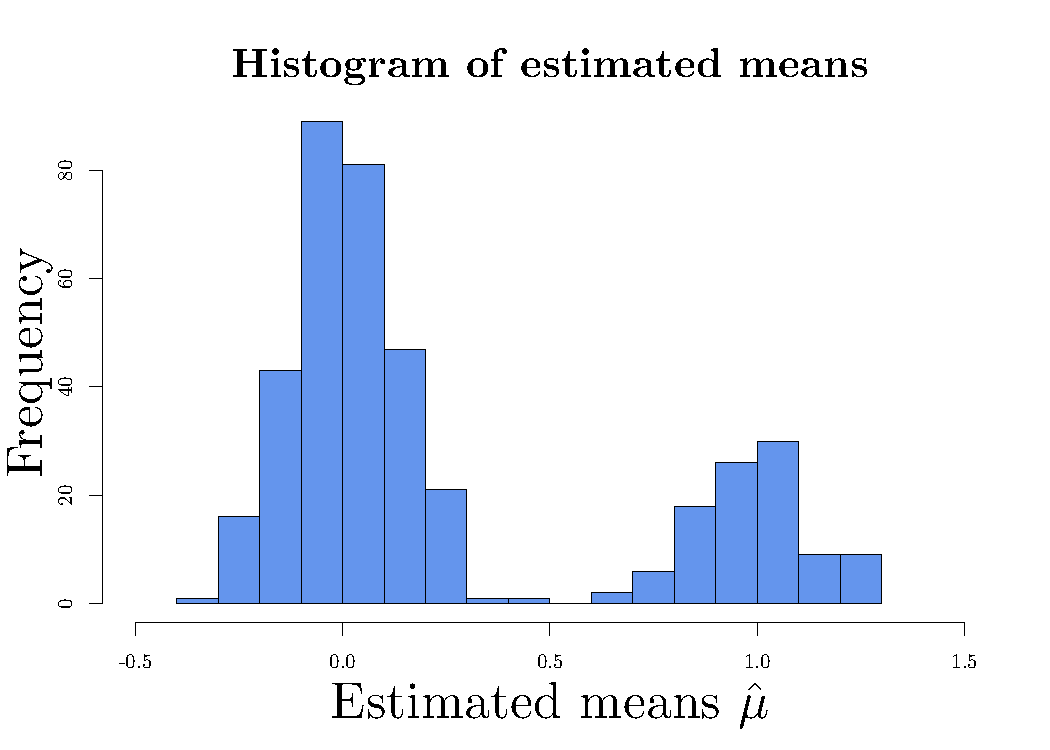
\includegraphics[width=.45\textwidth ]{figures/hist_mu.pdf}
                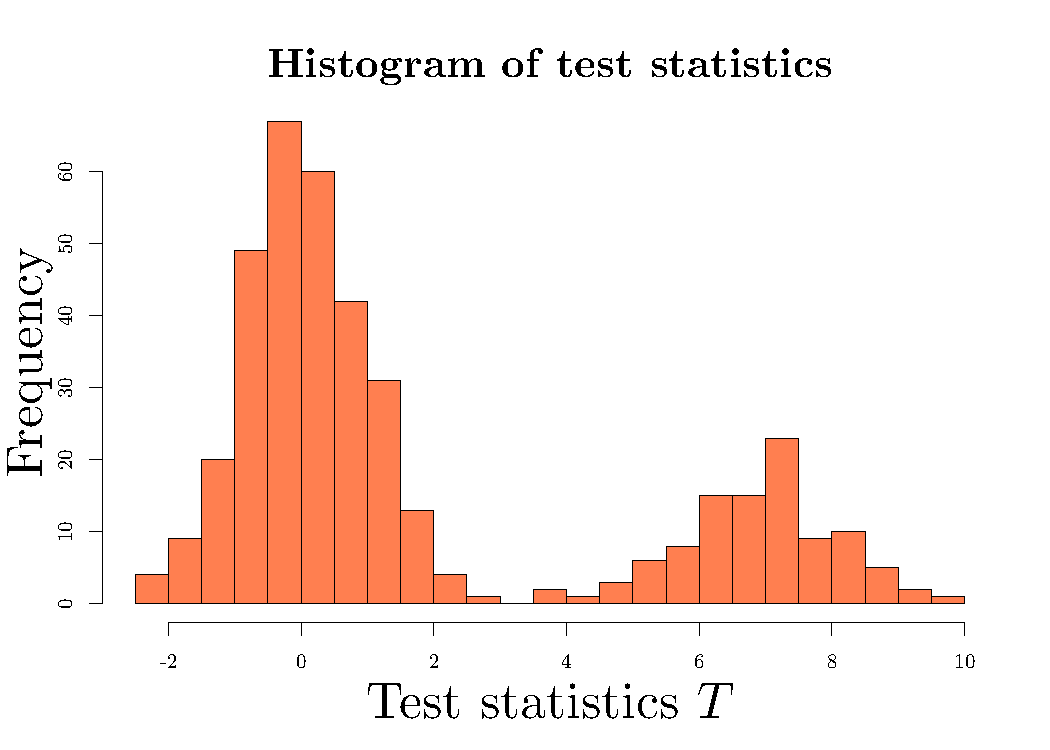
\includegraphics[width=.45\textwidth ]{figures/hist_stat.pdf} \\
                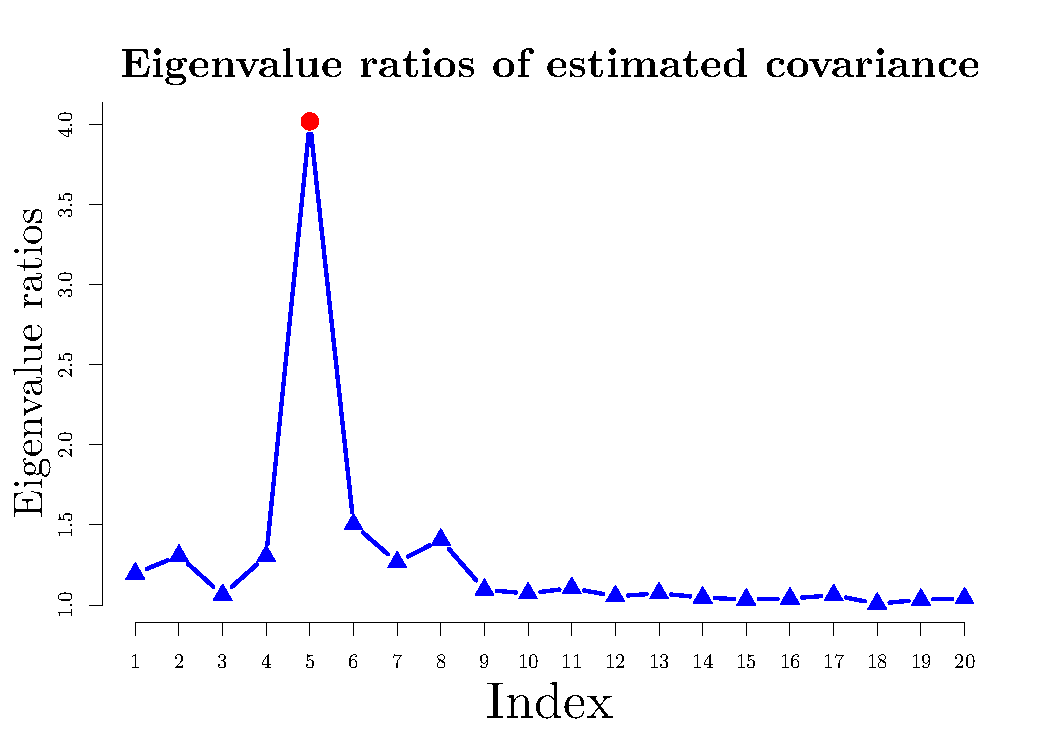
\includegraphics[width=.45\textwidth ]{figures/ratio.pdf}
                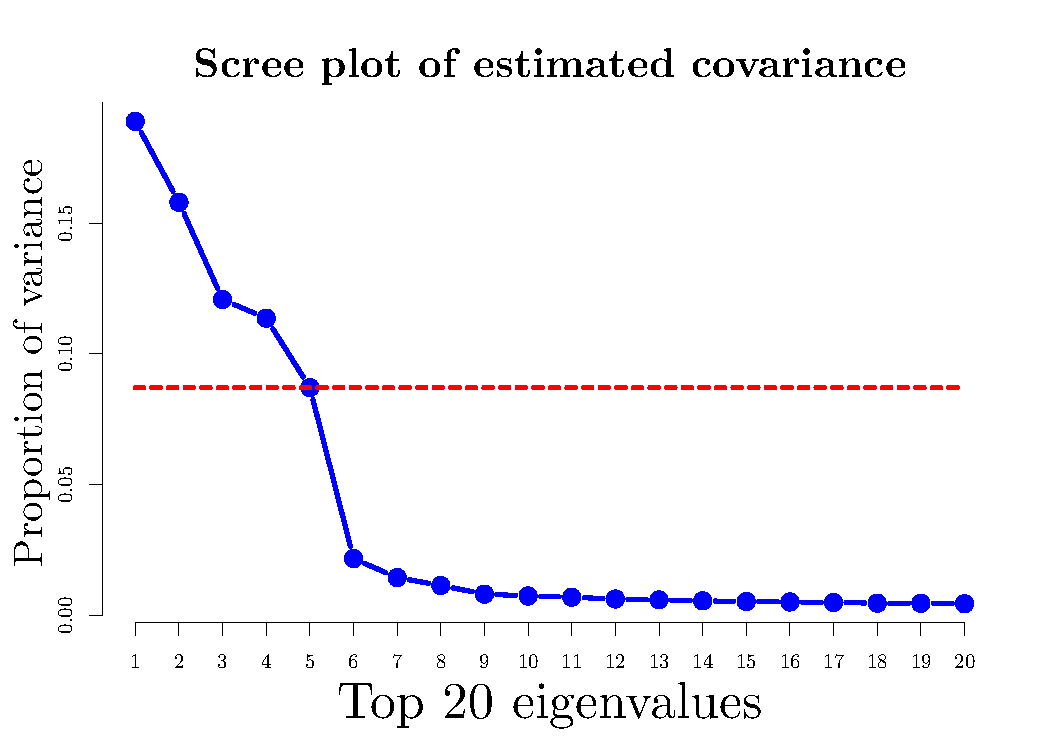
\includegraphics[width=.45\textwidth ]{figures/scree.pdf}
                \caption {Upper panel: histograms of estimated means and test statistics. Lower panel: eigenvalue ratio plot with the largest ratio highlighted and scree plot of the eigenvalues of the estimated covariance matrix.}
                \label{fig.plots}
\end{figure}




\subsection{Function call with options} \label{demo2}

In this section, we illustrate \code{farm.test} function with other options that allow us to call it more flexibly.
When the factors are observable, we can simply put the $n\times K$ factor matrix into argument \code{fX}, and the output is formatted the same as before. As a remark, among all the items listed in Table~\ref{output}, \code{eigenVal} and \code{eigenRatio}, which are eigenvalues and eigenvalue ratios of estimated covariance matrix, are not available in this case; see Algorithm~\ref{alg1}.

\begin{example*}
output <- farm.test(X, fX = FX)
output

One-sample FarmTest with known factors
n = 120, p = 400, nFactors = 5
FDR to be controlled at: 0.05
Alternative hypothesis: two.sided
Number of hypotheses rejected: 101
\end{example*}


Consider one-sided alternatives $H_{1j}: \mu_j \geq 0$, $j=1, \ldots p$ with a nominal FDR level $1\%$. We modify the arguments \code{alternative} and \code{alpha} as follows:


\begin{example*}
output <- farm.test(X, alternative = "greater", alpha = 0.01)
output

One-sample FarmTest with unknown factors
n = 120, p = 400, nFactors = 5
FDR to be controlled at: 0.01
Alternative hypothesis: greater
Number of hypotheses rejected: 101
\end{example*}


%\subsubsection*{None-zero null hypotheses}

Users can specify null hypotheses by passing any vector with length $p$ into argument \code{h0}. In the next example, we consider the $p$ null hypotheses as all the means are equal to $1$, so that the number of true nonnulls becomes $300$.


\begin{example*}
output <- farm.test(X, h0 = rep(1, p), alpha = 0.01)
output

One-sample FarmTest with unknown factors
n = 120, p = 400, nFactors = 5
FDR to be controlled at: 0.01
Alternative hypothesis: two.sided
Number of hypotheses rejected: 300
\end{example*}


%\subsubsection*{User-specified number of factors}

When the factors are unknown, users can also specify the number of factors based on some subjective grounds. In this case,  Step 3 in Algorithm~\ref{alg2} is avoided.
For example, we run the function with the number of factors chosen to be \code{KX = 2}, which is less than the true parameter $5$. This misspecification results in a loss of power with two true alternatives unidentified.


\begin{example*}
output <- farm.test(X, KX = 2)
power <- sum(output$reject <= p1) / p1
power

[1] 0.98
\end{example*}


As a special case, if we declare \code{KX = 0} in the function, a robust multiple test without factor-adjustment is conducted.


\begin{example*}
output <- farm.test(X, KX = 0)
output

One-sample robust multiple test without factor-adjustment
n = 120, p = 400
FDR to be controlled at: 0.05
Alternative hypothesis: two.sided
Number of hypotheses rejected: 95
\end{example*}



%\subsubsection*{Two-sample test}

Finally, we present an example of two-sample FarmTest. Using the same sampling distributions for the factor loading matrix, factors and noise vectors, we generate another sample $\left\{Y_i\right\}_{i = 1}^{m}$ from model \eqref{factor.model.twosample} with $m = 150$.

\begin{example*}
m <- 150
set.seed(200)
BY <- rustiefel(p, K) %*% diag(rep(sqrt(p), K))
FY <- rmvnorm(m, rep(0, K), diag(K))
uY <- rmvt(m, diag(p), 3)
Y <- FY %*% t(BY) + uY
\end{example*}

Then \code{farm.test} function can be called with an additional argument \code{Y}.


\begin{example*}
output <- farm.test(X, Y = Y)
output

Two-sample FarmTest with unknown factors
X.n = 120, Y.n = 150, p = 400, X.nFactors = 5, Y.nFactors = 5
FDR to be controlled at: 0.05
Alternative hypothesis: two.sided
Number of hypotheses rejected: 105
\end{example*}


The output is formatted similarly as in Table~\ref{output}, except that \code{means}, \code{stdDev}, \code{loadings}, \code{eigenVal}, \code{eigenRatio}, \code{nFactors} and \code{n} now consist of two items for samples \code{X} and \code{Y}. %In other words, to extract, say, estimated means of $\{X_i\}_{i = 1}^{n_1}$ from the output list, we have to apply dollar sign \code{$} twice.


\begin{example*}
names(output$means)

[1] "X.mean" "Y.mean"
\end{example*}





\section[Simulations]{Simulations}
\label{sec:testing}

In this section, we assess and compare the performance of \code{farm.test} function in the \pkg{FarmTest} package with the following methods:
\begin{itemize}
\item $t$-test using the R built-in function \code{t.test};
\item WMW-test  (\underline{W}ilcoxon-\underline{M}ann-\underline{W}hitney) using the \code{onesamp.marginal} function in the \pkg{mutoss} package;
\item RmTest (\underline{R}obust \underline{M}ultiple \underline{test}) without factor-adjustment by claiming \code{KX = 0} in the \code{farm.test} function.
\end{itemize}

For $t$-test and WMW-test, the functions we call produce vectors of p-values, to which the method proposed in \cite{S2002} is applied, see Steps 5--7 in Algorithm~\ref{alg1} or Steps 8--10 in Algorithm~\ref{alg2}.

 %and we further apply \code{farm.fdr} function in our package with these p-values as input to conduct multiple testing with FDR control. This additional step guarantees the fairness of this comparison.

In all the numerical experiments, we consider two-sided alternatives with a nominal FDR level $\alpha=5\%$. The true number of factors is  $5$. Factors and loadings are generated the same way as in \nameref{sec:data_generate} Section.
To add dependency among idiosyncratic errors, the covariance matrix of $\bu$, denoted by $\bSigma_u$, is taken to be a block-diagonal symmetric matrix with block size  $5 \times 5$. Within each block, the diagonal entries are all equal to $3$ and the off-diagonal entries are generated from $\mathcal{U}[0,1]$. {In the simulations, we drop the case where the generated $\bSigma_u$ is not positive-definite.}
The distribution of $\bu$ is specified in two models as follows.

\begin{itemize}
\item \textbf{Model 1}. $\bu \sim \cN\left(\mo, \bSigma_u\right)$: centered multinormal distribution with covariance matrix $\bSigma_u$;
\item \textbf{Model 2}. $\bu \sim  t_{3}\left(\mo, \bSigma_u\right)$: multivariate $t$-distribution with degrees of freedom 3 and covariance matrix $\bSigma_u$.
\end{itemize}

For each  model, we consider various combinations of sample size $n$ and dimensionality $p$, specifically, $n \in \left\{60, 80, 100, 120, 140\right\}$ and $p \in \left\{200, 400, 600, 800, 1000\right\}$. The number of true alternatives $p_1$ is taken to be $0.2\, p$, and the signal strength is set as $4 \sqrt{\log\left(p\right) / n}$.


Figures~\ref{fig:normal} and \ref{fig:T} depict the FDR and power curves for either "fixed $n$ growing $p$" or "fixed $p$ growing $n$" based on 200 simulations.
%are calculated based on $200$ independent Monte Carlo simulations, and they depict the tendency of FDP and power versus sample size and dimension for each method under two models.
Across various settings, FarmTest consistently maintains high empirical power with   FDR well controlled around the nominal level.
In contrast, the competing methods may lose as many as 10\% to 30\% powers, which can be ascribed to not accounting for the common factors.
%while other methods drop the power down to as low as $0.7$. Meanwhile, FarmTest, along with $t$-test and WMW-test, control the FDR fairly successfully, with empirical FDP slightly above the desired level, but RmTest exhibits the highest FDP in almost every experiment.
 In summary, we conclude that the \pkg{FarmTest} package provides an efficient implementation of the FarmTest method, which carries out multiple testing for multivariate data with heavy-tailed distribution and a strong dependency structure.

 % implemented in \code{FarmTest} package is suitable for application in a wide range of settings since it provides adequate FDR control while achieving high power, even when the data carry one of the following ill characters: (1) heavy-tailedness; (2) strong dependence; (3) large dimension and small sample size; and (4) low signal-to-noise ratio.

\begin{figure}[!t]
\centering
                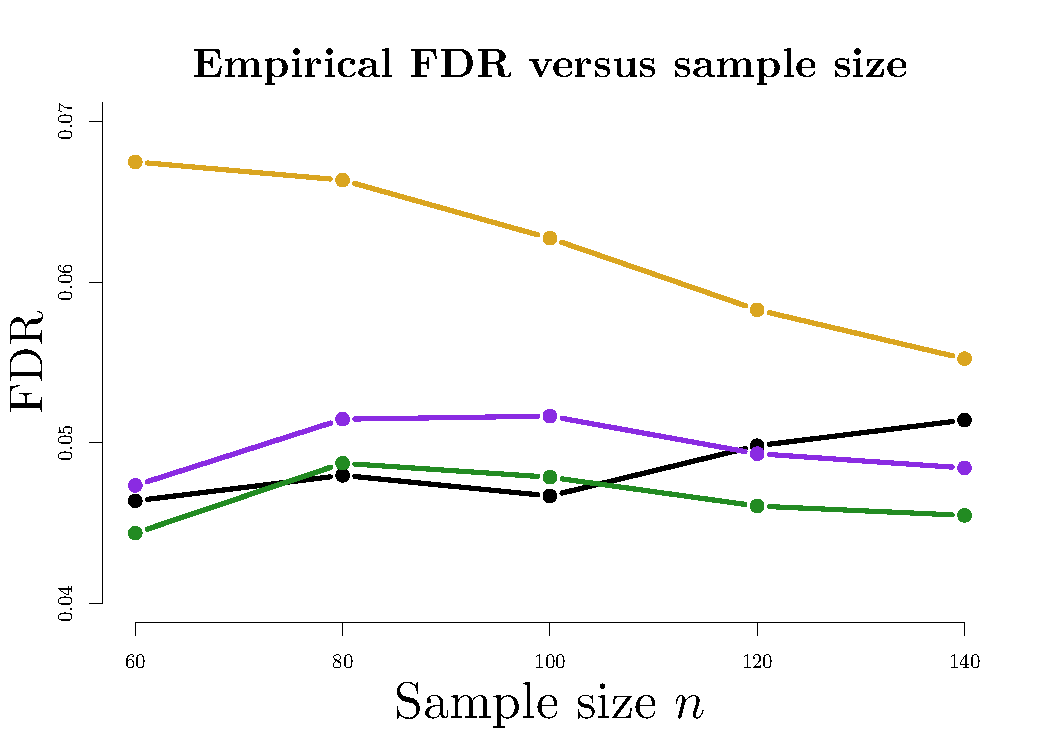
\includegraphics[width=.45\textwidth ]{figures/FDP_normal_fixp.pdf}
                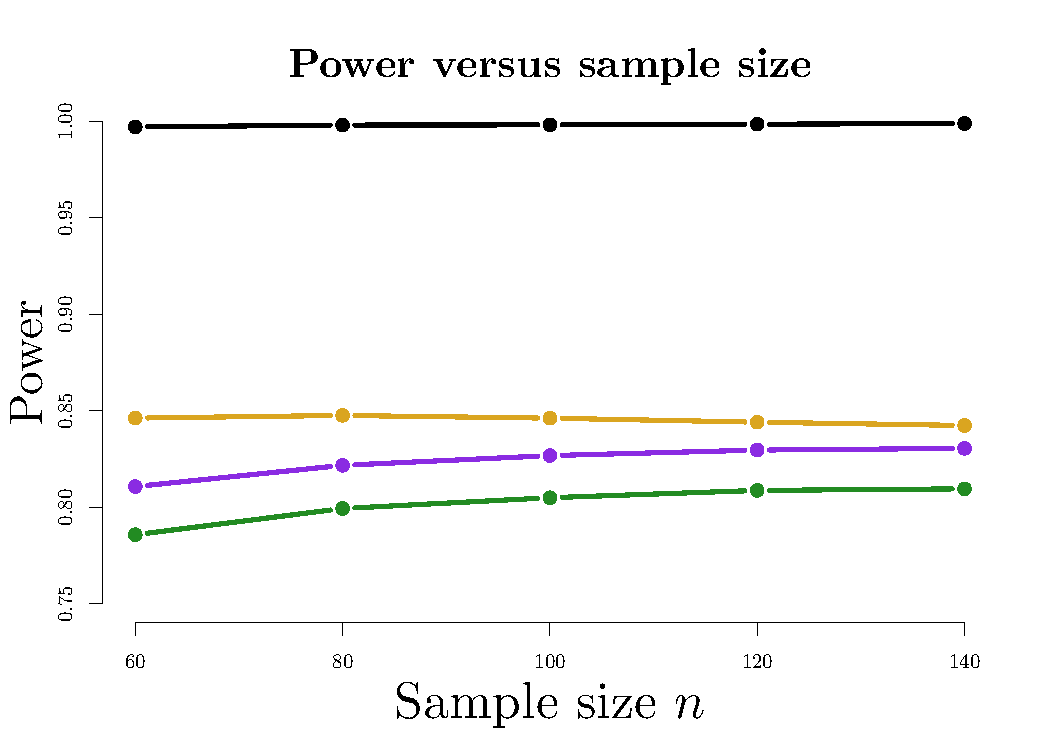
\includegraphics[width=.45\textwidth ]{figures/Power_normal_fixp.pdf} \\
                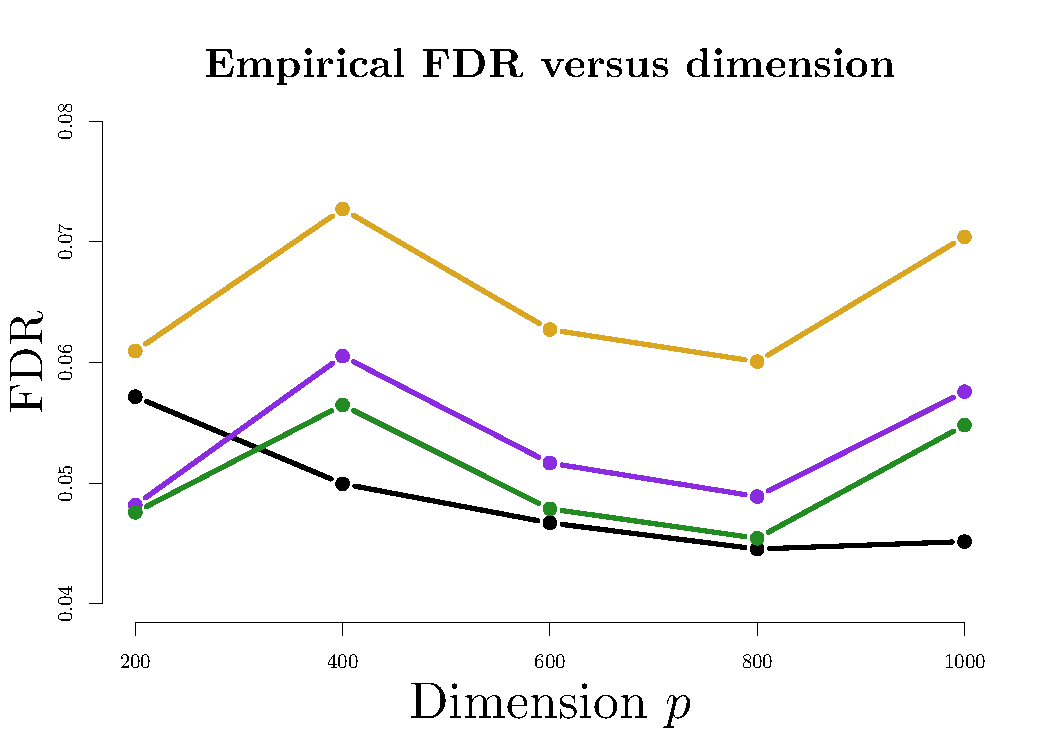
\includegraphics[width=.45\textwidth ]{figures/FDP_normal_fixn.pdf}
                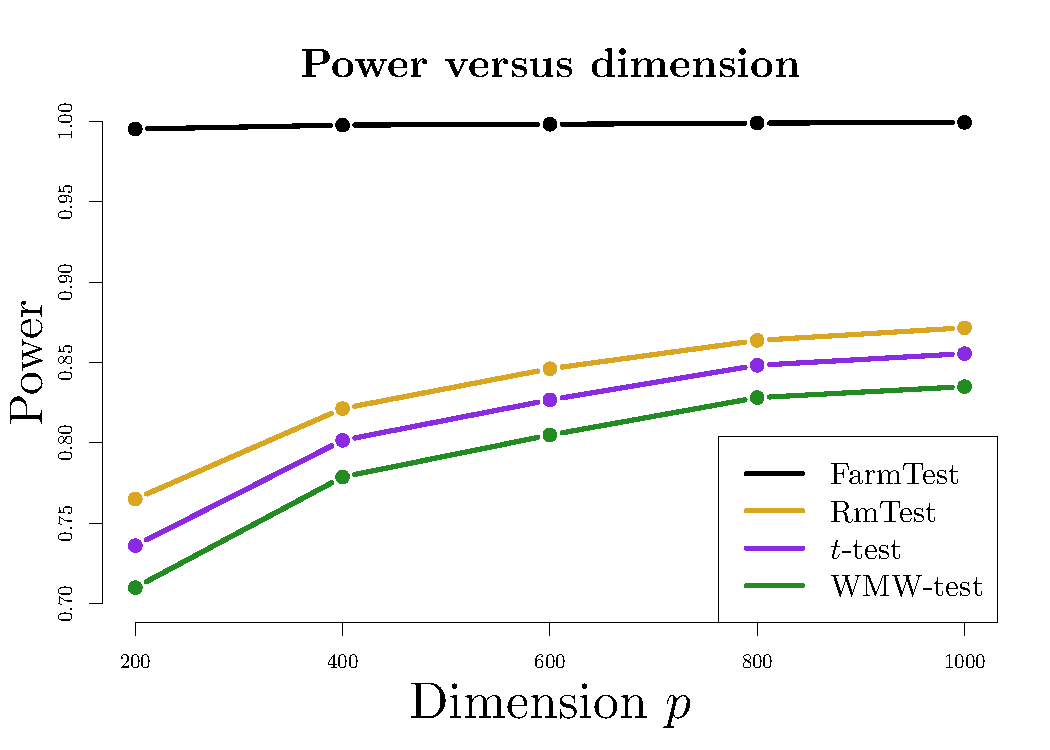
\includegraphics[width=.45\textwidth ]{figures/Power_normal_fixn.pdf}
                \caption {Comparison of {FarmTest} with three other methods in terms of FDR and power under Model 1 (multivariate normal distribution). In the upper panel,  $p$ is fixed at $600$ and $n$ grows from 60 to 140; in the lower panel, $n$ is fixed at $100$ and $p$ ranges from 200 to 1000.}
                \label{fig:normal}
\end{figure}


\begin{figure}[!t]
\centering
                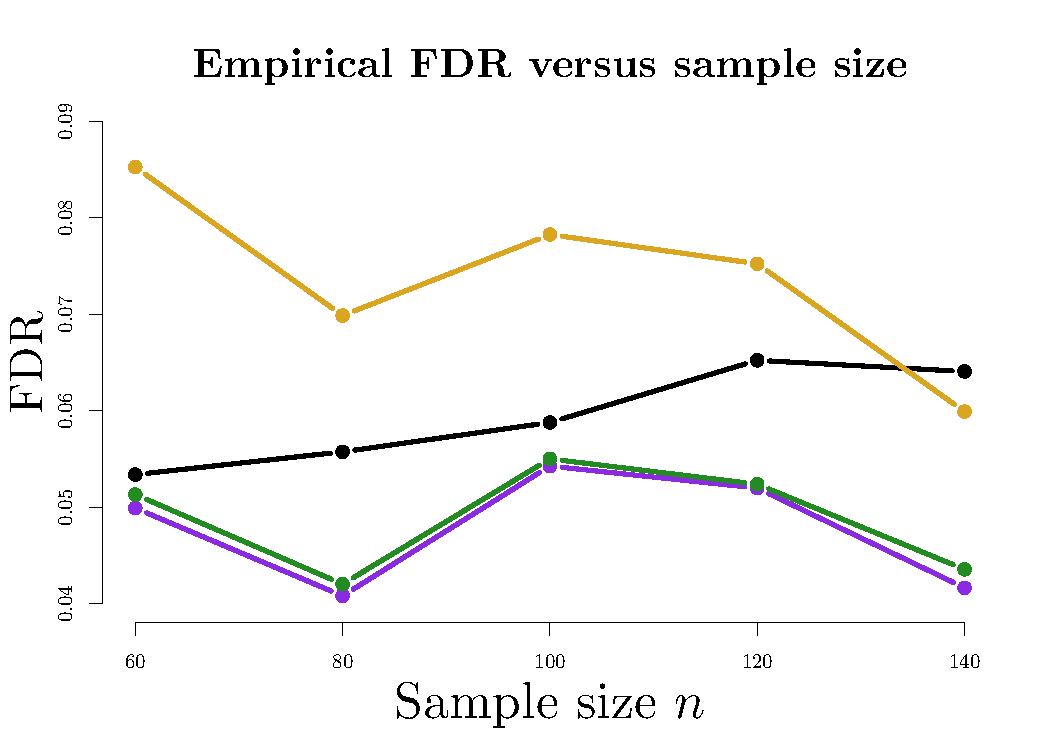
\includegraphics[width=.45\textwidth ]{figures/FDP_T_fixp.pdf}
                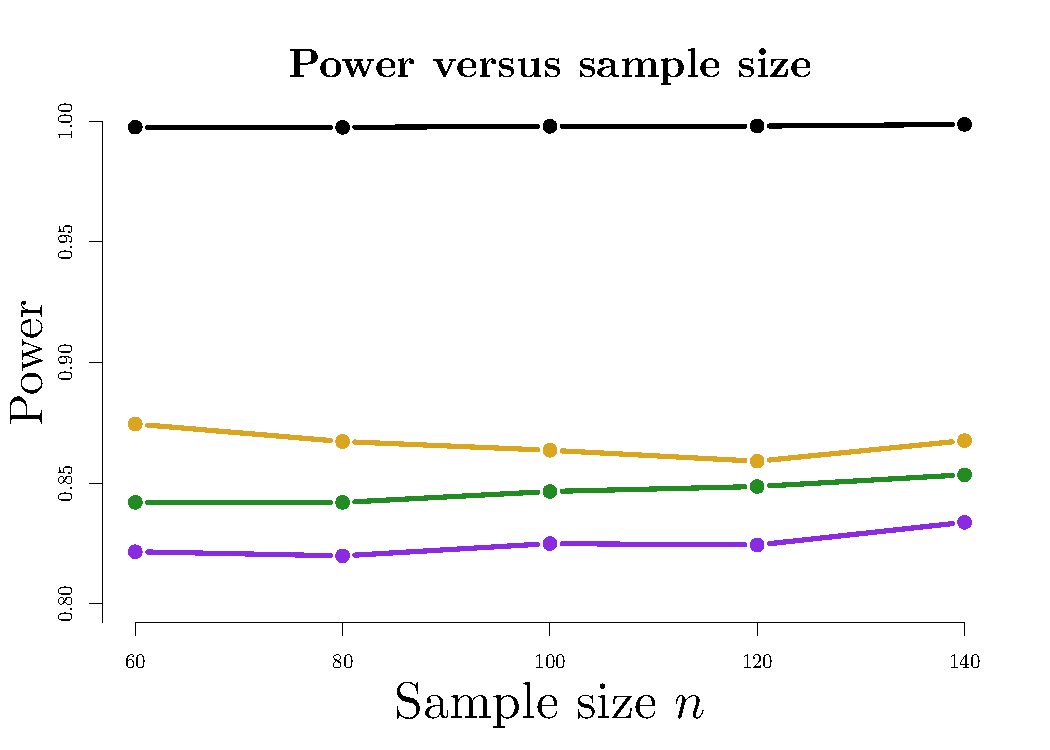
\includegraphics[width=.45\textwidth ]{figures/Power_T_fixp.pdf} \\
                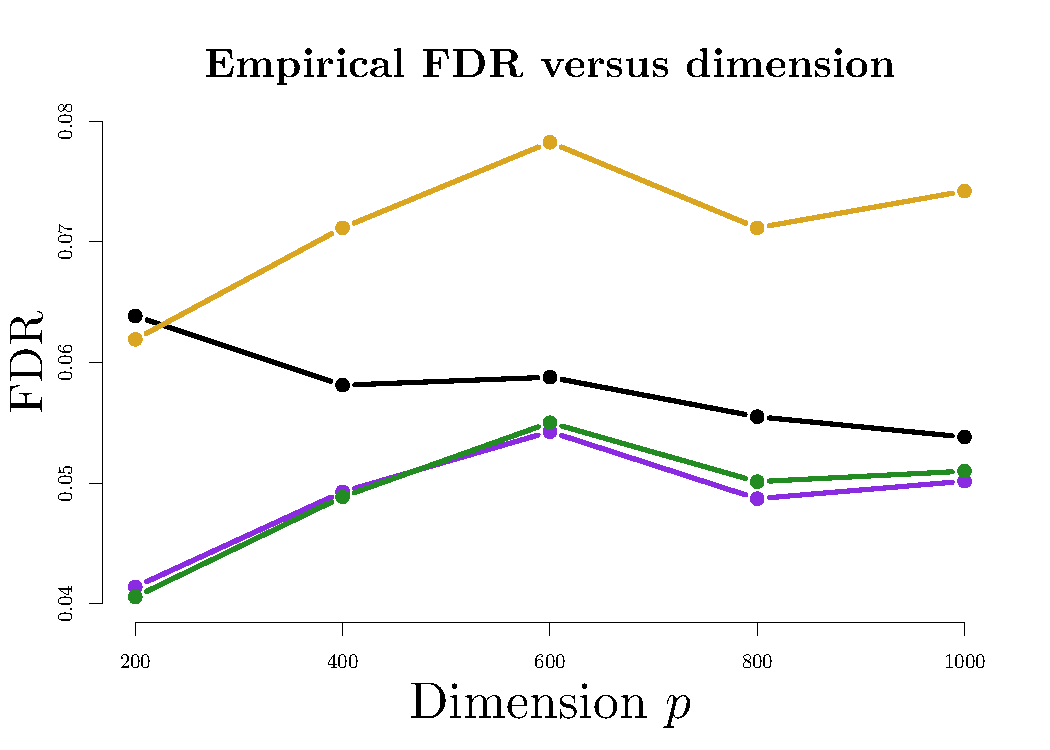
\includegraphics[width=.45\textwidth ]{figures/FDP_T_fixn.pdf}
                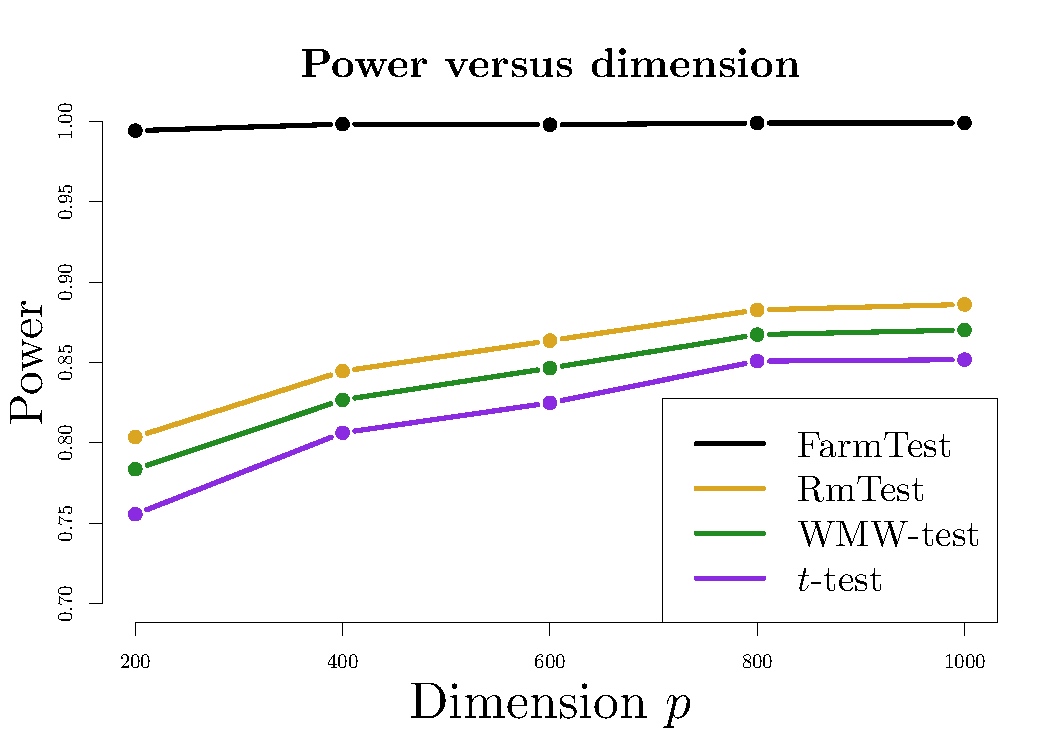
\includegraphics[width=.45\textwidth ]{figures/Power_T_fixn.pdf}
                \caption {Comparison of {FarmTest} with three other methods in terms of FDR and power under  Model 2 (multivariate $t$-distribution). In the upper panel, $p$ is fixed at $600$ and $n$ grows from 60 to 120; in the lower panel, $n$ is fixed at $100$ and  $p$ ranges from 200 to 1000.}
                \label{fig:T}
\end{figure}


\section{Real data example}\label{sec:real_data}


In this section, we apply the \pkg{FarmTest} package to test the mean effects of stock returns.  In capital asset pricing theory, the stock's risk-adjusted mean return or "alpha" is a quantity of interest since it indicates the excessive return incurred from investing in a particular stock. If the efficient equity market hypothesis holds, we expect "alpha" to be zero. Hence, detecting non-zero alphas can help investors to identify market inefficiencies, that is, whether certain stocks exhibit an abnormal rate of return or are mispriced. As discussed in \cite{C2001}, both cross-sectional dependency and heavy tailedness are silent features of stock returns. 
%Traditional multiple testing tools may fail to efficiently detect true non-zero alphas while keeping the false discovery rate under control.

%When the market is inefficient, we can conduct multiple hypothesis testing to identify those stocks in the market that have statistically significant alphas, while correcting for risk or volatility incurred by the stock.

In this study, we test the annual mean effects of stocks in the S\&P500 index. The data is available on COMPUSTAT and CRSP databases. %Figure~\ref{fig:stocks_kurtosis} displays the histogram of 
We find that most of  the stocks with continuous membership in the S\&P500 index from 2008 to 2016 have excess kurtosises greater than zero, indicating tails heavier than that of a normal distribution. 
Also, more than $33\%$ of the stocks are severely heavy-tailed as their excess kurtosises exceed 6, which is the excess kurtosis of $t_5$-distribution.
We collect monthly returns of stocks from the S\&P500 index over rolling windows: for each month between 2008 and 2016, we collect monthly returns of stocks who have continuous records over the past year. The average number of stocks collected each year is 598. For each rolling window, we conduct multiple testing using the four methods considered in the previous section, that is, FarmTest, $t$-test, WMW-test, and RmTest.

The nominal FDR level is set as $\alpha=1\%$. Within each rolling time window, we have $p \approx 600$ and $n=12$. The numbers of discoveries of each method are depicted chronologically in Figure~\ref{fig:stocks}, and Table~\ref{tab:stocks} displays several key summary statistics.
Since the $t$-test barely discovers any stock throughout the whole procedure, we only present the results for the other three methods in Figure~\ref{fig:stocks}.
It is interesting to observe that across different time rolling windows, the testing outcomes of the WMW-test are relatively stable and time-insensitive. FarmTest, on the other hand, selects much fewer stocks in the year of 2009, coinciding to some extent with the financial crisis during
which the market volatility is much higher.
%The test results show that, for each year, FarmTest selects more mispriced stocks than the $t$-test and WMW-test.
RmTest typically selects the most stocks, which is partly due to the lack of FDR control under strong dependency.
A major, noticeable impact of dependence is that it results in clusters of rejections: if a test is rejected, then there are likely to be further rejections for tests that are highly correlated with this one.
%who exhibit statistical significance than the other three conservative methods without dependence-adjustment.
% In particular, $t$-test doesn't detect any significance during the whole procedure.
This phenomenon is in accord with our simulation results, showing that FarmTest simultaneously controls the FDR and maintains high power while the other methods either make too many false discoveries or fail to detect true signals.

\iffalse
 All the data in this section was obtained from the COMPUSTAT and CRSP databases at the Wharton Research Data Services engine. We use monthly returns between 2005 to 2016 for all stocks included in the S\&P500 index. For each year, we only use those stocks that have continuous inclusion in the index, resulting in an average of $602$ stocks every year. In Figure~\ref{fig:stocks_kurtosis} we show the kurtosis of all the stocks, which show that we indeed have very heavy-tails in the data. $30\%$ of the stocks exhibit a kurtosis larger than 10, whereas the normal distribution has a kurtosis of $0$ and the heavy-tailed $t_5$ distribution has a kurtosis of $6$.

For each year, we test the hypotheses that the mean return of each stock is zero with   FDR controlled at  $\alpha=5\%$. Figure~\ref{fig:stocks} summarizes the number of discoveries using the proposed method, compared with others. We see that out of the entire portfolio, only a few stocks exhibit statistically significant alphas. The non-robust method selects a large number of stocks, which are possibly false discoveries. The methods with no dependence adjustment select very few stocks, exhibiting low power which is in agreement with the simulation results.
\fi

 
%\begin{figure}[!t]
%\centering
%\includegraphics[width=.7\textwidth]{figures/Fig_real_1.pdf}
%\caption {Histogram of excess kurtosises of monthly returns of the stocks in the S\&P500 index from 2008 to 2016. The red dashed line marks the excess kurtosis of $t_5$-distribution.}
%\label{fig:stocks_kurtosis}
%\end{figure}


\begin{figure}[!t]
\centering
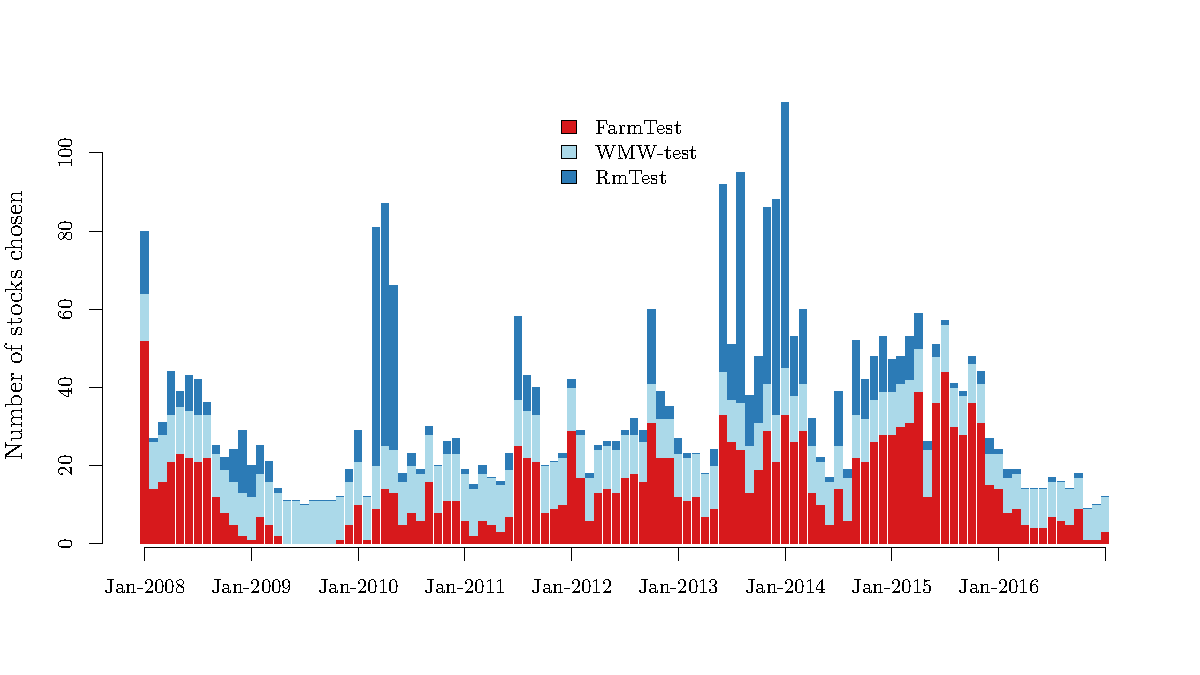
\includegraphics[width=.7\textwidth]{figures/Fig_real_2.pdf}\\
\caption {Stack bar plot of the numbers of discoveries via {FarmTest}, WMW-test and RmTest from 2008 to 2016, using rolling windows of one year. Within each time window, we report the number of stocks in the S\&P500 index that show significant statistical evidence against null hypotheses that there are no excessive returns,  with FDR controlled at $1\%.$}
\label{fig:stocks}
\end{figure}


\begin{table}[tbh]\centering
%\footnotesize{\begin{tabular}{lccccc}
{\begin{tabular}{l|ccccc}
\hline \vspace{-0.25cm} \\
  Method&Mean & Std. Dev.&Median &Min &Max \vspace{0.1cm} \\
 \hline  \vspace{-0.3cm}  \\
\color{blue}FarmTest &\color{blue}14.477 &\color{blue}11.070 &\color{blue}12 &\color{blue}0&\color{blue}52\\
%$t$-test &0 &0&0&0&0\\
WMW-test &10.991 &1.005&11&8&12\\
RmTest&8.147 & 14.414&3&0&68\\\hline
\end{tabular}
\caption{Summary statistics of the number of discoveries via {FarmTest}, WMW-test and RmTest between 2008 and 2016 using rolling windows of size 12 (months).}
\label{tab:stocks}}
\end{table}





\section[Summary]{Summary}\label{sec:discussion}
We provide an R package to implement {FarmTest}, a flexible large-scale multiple testing method that is robust against strongly dependent and heavy-tailed data. The factor-adjustment procedure helps to construct weakly dependent test statistics, and also enhances statistical power by reducing the signal-to-noise ratio. Moreover, by exploiting the idea of adaptive Huber regression, the testing procedure is robust against heavy-tailed noise. The efficacy of our package is demonstrated on both real and simulated datasets.















\bibliography{FarmTestRJ}




\address{Koushiki Bose, Jianqing Fan\\
  Department of Operations Research and Financial Engineering\\
  Princeton University, Princeton, NJ 08544\\
  USA\\
  \email{koush.bose@gmail.com}, \email{jqfan@princeton.edu}}

\address{Yuan Ke\\
  Department of Statistics\\
  University of Georgia, Athens, GA 30602\\
  USA\\
  \email{Yuan.Ke@uga.edu}}
  
\address{Xiaoou Pan, Wen-Xin Zhou\\
  Department of Mathematics\\
  University of California, San Diego, La Jolla, CA 92093\\
  USA\\
  \email{xip024@ucsd.edu}, \email{wez243@ucsd.edu}}



\end{article}

\end{document}
